%!TEX root=../tax-democracy-held.tex

%add comments, footnote:
%this was first submitted as \ldots

\begin{quote}
	\emph{``Yes we can:
	to justice and equality.
	Yes we can:
	to opportunity and prosperity.''}
	\\*
	--- Barack H.\ Obama, Obama For America 2008
\end{quote}

\section{The Contestants}
	\label{sec:contestants}
Which taxes exist in the real world, and which taxes are conceivable?
It will not be possible to list them all here in all their legal and administrative detail.
Instead, rough archetypes of real existing taxes (\gls{vat}, \gls{payroll}, (Dual) \gls{pit}, \gls{cit}, \gls{lbt}) will serve to compare them to the three hypothetical (or rare) taxes suggested (\gls{pct}, \gls{wt}, \gls{nit}).

%also explain the distinction of indirect taxes here, because I don't use that in the following, it's more analytic than that.

%here used to be the tax-overview thing, it's now in testing-hypotheticals

\begin{figure}[htbp]
	\centering
	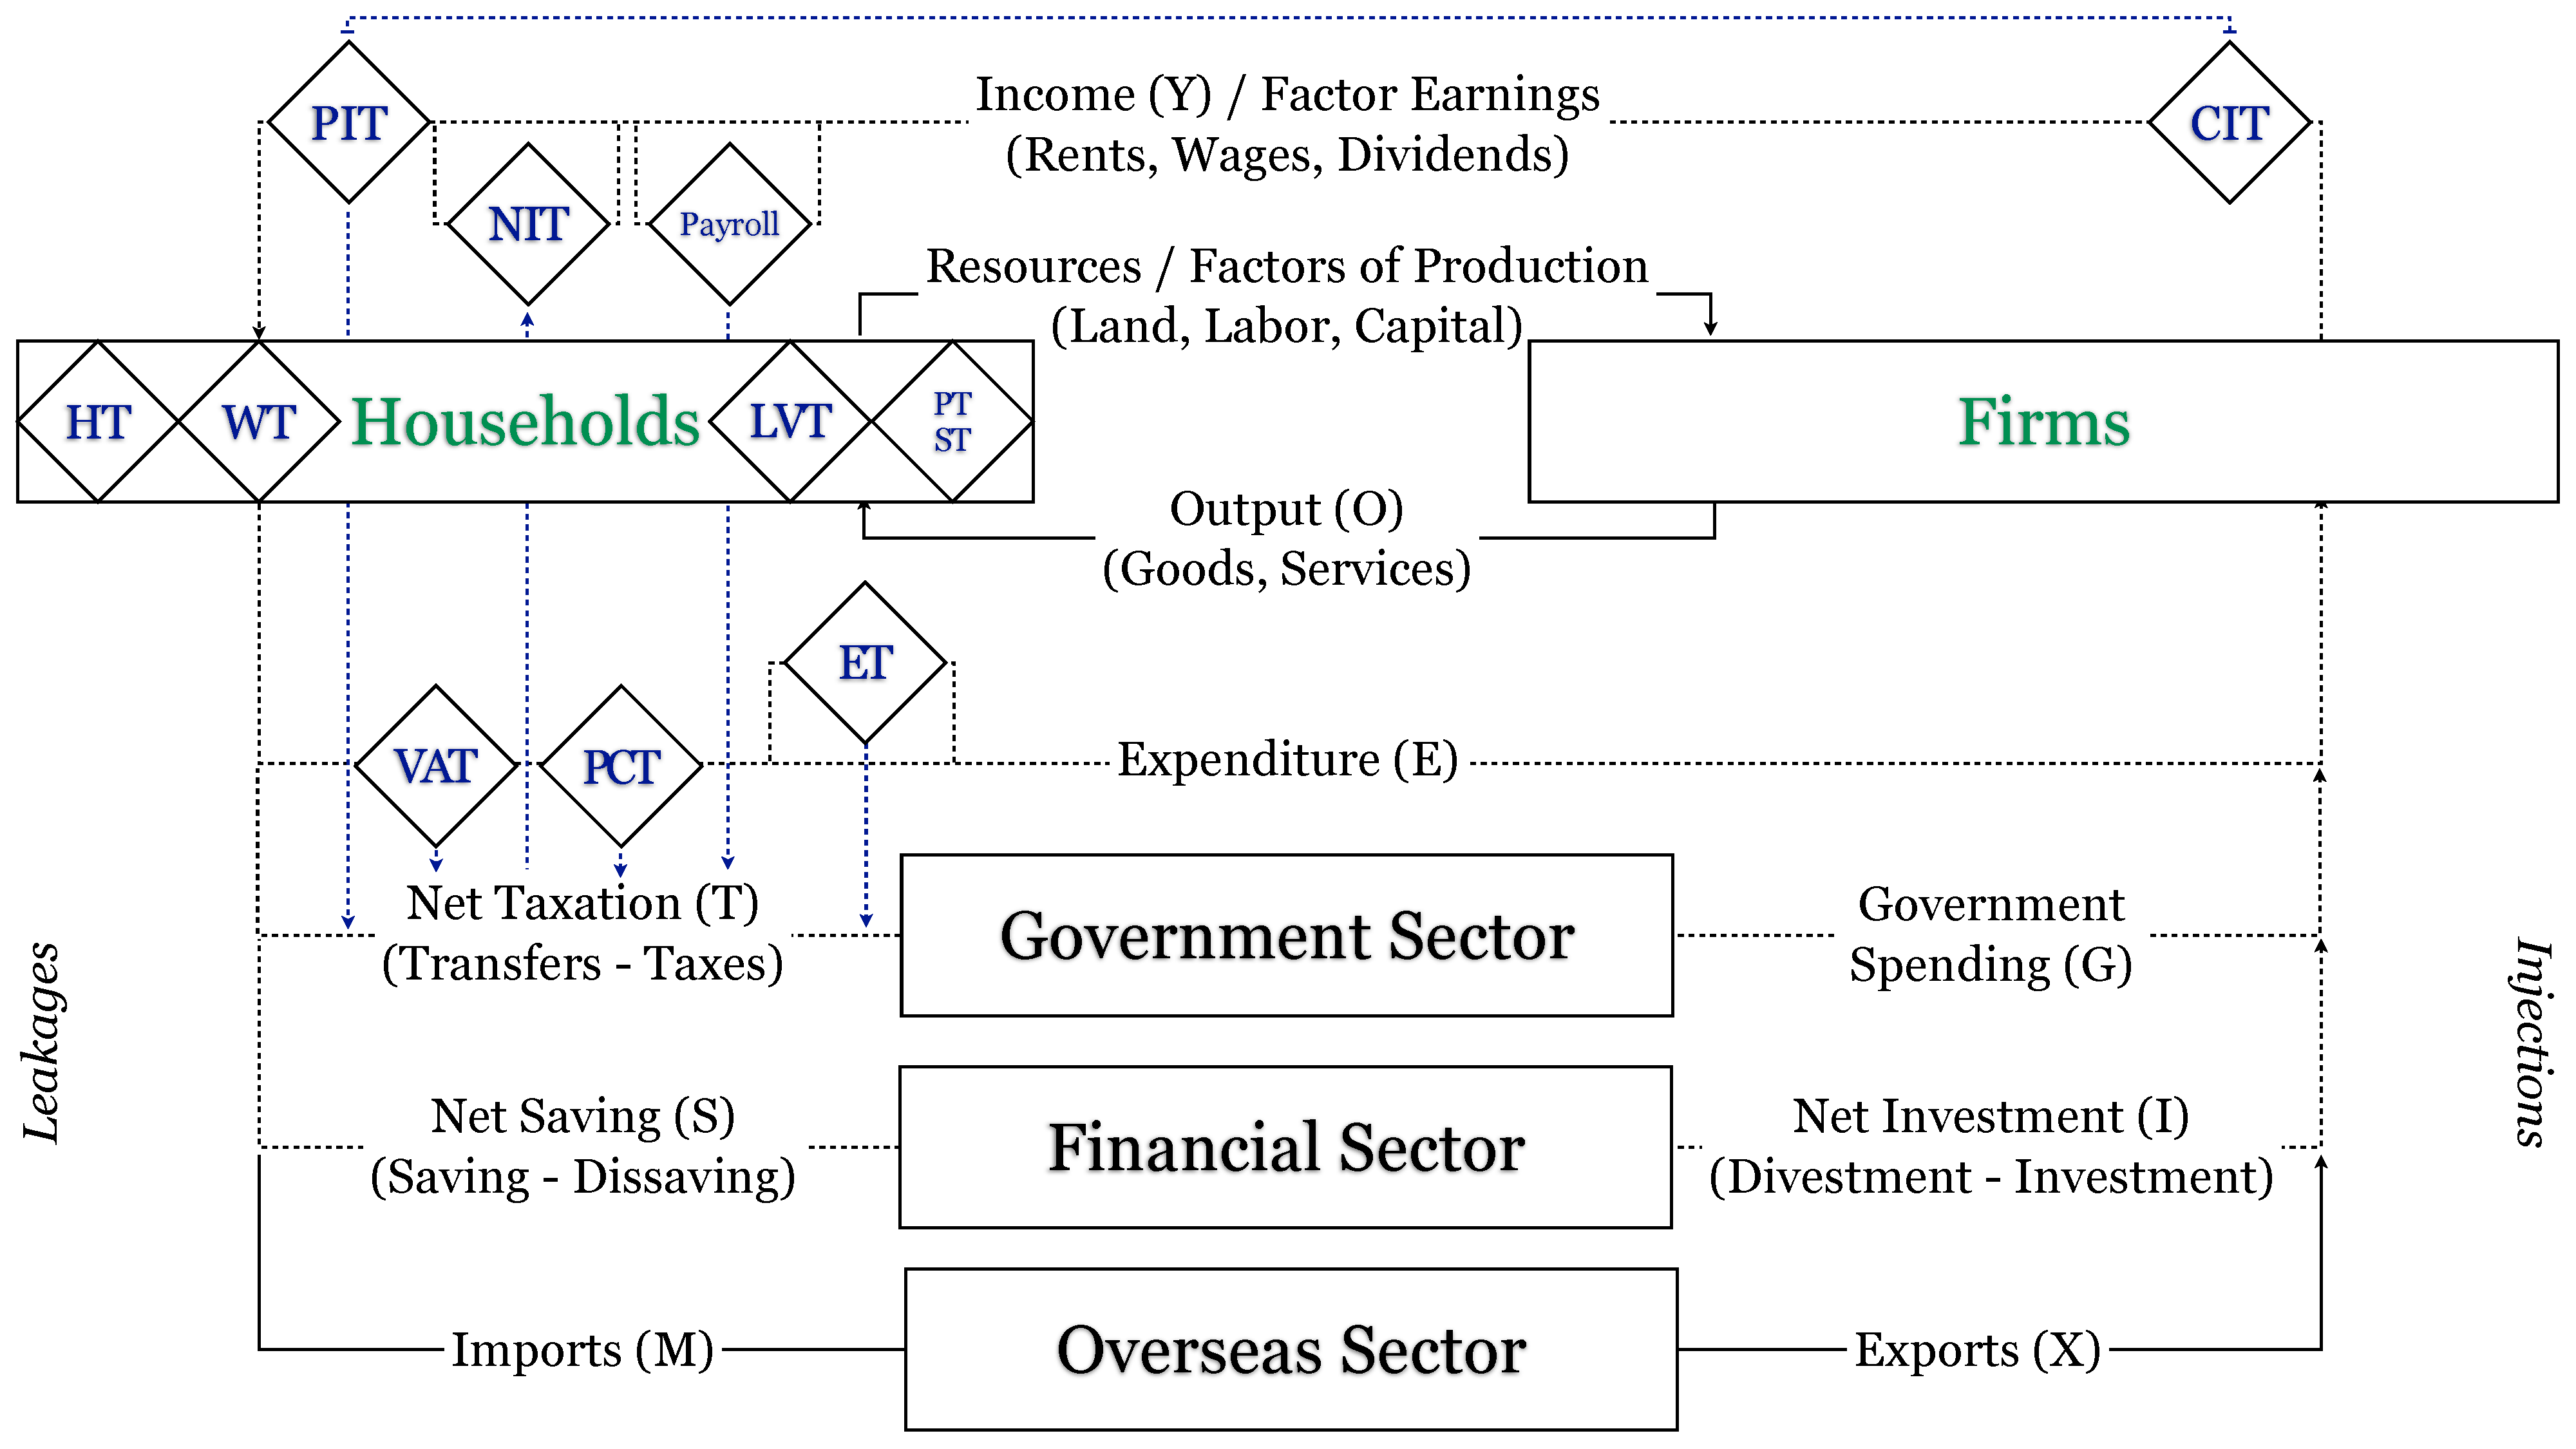
\includegraphics[width=1\textwidth]{circular-flow-with-taxes}
	\caption[Circular Flow in the Economy, with Taxes]{Circular Flow of Income in the Economy, with Tax Revenue Sources}
	\begin{flushleft}
		\scriptsize{Compare \autoref{fig:circular-flow}.}
		%!TEX root=../tax-democracy-held.tex

\scriptsize{
	\glsfirst{CIT},
	\glsfirst{Dual-PIT},
	\glsfirst{Ecotax},
	\glsfirst{ET},
	\glsfirst{FTT},
	\glsfirst{LBT},
	\glsfirst{LVT},
	\glsfirst{NIT},
	\glsfirst{OSN},
	\glsfirst{PCT},
	\glsfirst{Payroll},
	\glsfirst{PT},
	\glsfirst{SD},
	\glsfirst{VAT},
	\glsfirst{WT},
	\glsfirst{Y2C} and

	\hyperref[sec:distributive-effects-of-inflation]{the distributive effects of in- and deflation} (p.~\pageref{sec:distributive-effects-of-inflation}).
}
	\end{flushleft}
	\label{fig:circular-flow-with-taxes}
\end{figure}
%comment on the extra loops for some taxes

Enter the contestants.

\subsection{Head Tax}

\subsection{Taxes on Income}

\subsubsection{Taxes on Capital Income}

\paragraph{Corporate Income Tax (CIT)}
	\phantomsection
	\label{sec:CIT}
The \glsreset{cit} \gls{cit} taxes the earnings
\footnote{
	In Germany, earnings after interest, depreciation and amortization.
}
of an incorporated firm.
It is usually proportional.
Unincorporated firms do not pay \gls{cit}, instead their owners owe \gls{pit} on their business earnings.
\footnote{
	When a corporation hands out a dividend, the dividend is also \gls{pit}ed.
	In some jurisdictions, \gls{cit} is deductible from the \gls{pit} on dividends.
	No taxation of dividends applies when the recipient is another corporation.
}
%Graetz 1979:
%1635 makes my key point:
%the one reason for CIT is that "undistributed corporate income does not escape taxation"
	%abolish business taxation (1636)
	%a corporation has no one "ability to pay"

\glspl{cit} are proportional, with rates around 20\% in the EU.
Countries have recently created issued sectoral (trade, finance) or regional (Hong Kong, London) exemptions from the \gls{cit} to attract investment \citep{Genschel2009,Ganghof2007,Genschel2005}.

\subparagraph{Local Business Tax (LBT)}
	\phantomsection
	\label{sec:LBT}
Taxes on local businesses exist only in some OECD countries, including Germany.
In Germany, local authorities can tax local business a progressive tax on their earnings.
Local authorities set the rate of the tax (within federally mandated margins).
Firms are taxable based on the location of their establishments.
Earnings of firms with multiple establishments are weighed by the sum of wages and salaries paid.

\subsubsection{Taxes on Capital and Labor Income}

\paragraph{Personal Income Tax (PIT)}
	\phantomsection
	\label{sec:PIT}
Under the \glsreset{pit} \gls{pit}, all sources of personal income (labor, capital) are added and taxed under a single schedule.
\gls{pit} schedules are typically progressive.
Marginal (not average!) tax rates in Germany range from 14\% to 42\% (Bundesministerium für Finanzen 2009).
%better quote

	%The personal income tax is usually levied according to a progressive schedule both on labor and capital income.
%Its incidence is borne by the taxed individual, but it disincentivizes work and (risky) investment.
%It taxes capital twice:
%once when it is initially earned and again when it generates an interest.
%Income taxes only on labor (payroll tax, social contributions) can contribute to structural unemployment by raising effective price floors, especially when they are not sufficiently progressive.

	%Personal income taxes on capital (\ldots
%gains tax) necessitate a corollary taxation of corporate income.
%Without it, taxpayers could easily evade payment by incorporating capital it in a firm, withdrawing earnings only slowly.
%Corporate income tax rates spill over to personal (capital gains) tax rates (Ganghof & Genschel 2008, Ganghof 2006).
%Like the personal income tax, they depress economic activity.
	%Moreover, corporate income taxes are indeterminate with regard to incidence and flat in their progression.
%The tax incidence in a firm on either labor or capital is determined by a host of firm- and market-specific factors, including the relative factor price elasticities.
%Corporate income taxes apply one rate over all shares.
%The lifesavings of a worker, invested in a company through her life insurance, are taxed at exactly the same rate as the share of a stock-market tycoon.
	%As the base of the corporate income tax is relatively mobile (compared to labor, consumption), it can easily evade taxation or compete down rates.

\subparagraph{Dual Income Tax (Dual PIT).}
	\phantomsection
	\label{sec:Dual-PIT}
\glsreset{2-pit} The \gls{2-pit} is a variation on the \gls{pit}, where schedules differ between capital and labor sources of income.
\glspl{2-pit} burden capital relatively less than labor incomes.
The \glspl{2-pit} was introduced to avoid the negative growth effects of high capital taxation (particularly through its \hyperref[sec:CIT]{CIT backstop}, p.~\pageref{sec:CIT}) and to counteract capital flight.

In Sweden, a pioneer of the \gls{2-pit}, the top marginal (not average!) rate for labor incomes is 55\%.
Capital incomes are taxed proportionally at 30\% (marginal rate equals average rate).
%add reference

\subsubsection{Taxes on Labor Income}

\paragraph{Payroll Taxes (Payroll)}
	\phantomsection
	\label{sec:Payroll}
In Germany, and many other countries, social contributions for old age, health, unemployment and long term care insurance are implemented as payroll taxes.
Payroll taxes are paid on labor income.
Whether they are implemented as withholding taxes (the employer withholds and transfers the tax) or paid out of the employees funds is of no significance here:
it does not matter for \hyperref[sec:tax-incidence]{tax incidence} (page \pageref{sec:tax-incidence}).

\subparagraph{Social Insurance Contributions}
	\phantomsection
	\label{sec:SIC}
are capped \glsreset{payroll} \gls{payroll}, actually.
Despite this terminological confusion and their administration in semi-independent public agencies, it is important to note that social contributions are government revenue, irrespective of their quasi-fiscal status.
Social contributions are proper pages
	%ref missing, defunct
	% \hyperref[sec:PurposesOfTaxation]{proper taxes} (page \pageref{sec:PurposesOfTaxation}).}
To the extent that government adopts universal provision of health care, unemployment insurance and long term care as allocative goals, compulsory contributions to these services are \hyperref[sec:fiscal-redistribution]{redistributive taxes}.
To the extent that government finances old-age pensions out of current incomes, such PAYGO contributions are intertemporally and intergenerationally redistributive taxes.
	%href defuct
	%\hyperref[sec:fiscal-redistribution]{redistributive taxes}.
\footnote{
	Payments into capital-based pension schemes are not straightforwardly taxes.
	Government may however choose to mandate or subsidize such payments to increase the savings rate.
	%below is defunct
		%As per desideratum \ref{des:Savings} (\hyperref[des:Savings]{arbitrary savings rate}, page \pageref{des:Savings}) such a market intervention \emph{would} be a proper tax, too.
}
To the extent that private markets for health care, unemployment and long term care insurance are plagued by lemons markets \citep{Akerlof-1970-aa}, respective contributions serve to \hyperref[sec:state-insurance]{pool risks} (page \pageref{sec:state-insurance}) and are proper revenue-generating taxes.
Additionally, universal health care provides \hyperref[sec:public-good]{public good} provision against epidemics (think vaccinations) and unemployment insurance serves as an automatic stabilizer to smooth out economic growth.
	%ref defunct
	% \hyperref[des:AutomaticStabilizer]{automatic stabilizer} (page \pageref{des:AutomaticStabilizer}) to smooth out economic growth.

Social insurance contributions are presented here for the sake of completion and clarification.
They are, when typically implemented as payroll taxes, a variation of a \gls{2-pit}.

Rates for social insurance contributions are usually proportional.
In the EU, they vary from 20\% in Denmark to 32\% in Germany and 50\% in France (Statistisches Bundesamt Deutschland 2007).
In Germany, contributions are capped above a certain income threshold, above which additional income is not taxed.

\subsection{Taxes on Consumption}

%what about the distinction about INDIRECT taxes.
%Indirect taxes are taxes levied on entities other than those expected to bear the eventual burden.

\subsubsection{Prepaid Consumption Taxes}

\paragraph{Value Added Tax (VAT)}
	\phantomsection
	\label{sec:VAT}
The \glsreset{vat} \gls{vat} is best understood as an elegant advancement of a retail sales tax.
%best example for a prepaid consumption tax is VAT, in the american context sales taxes
A retail sales tax charges sellers a fixed percentage of the sales price on goods for which the (corporate or private) buyer is the end user.
Because under a sales tax, the tax on any single taxable transaction is very high, incentives to evade the tax and to smuggle goods are great.
What is more, the state looses \emph{all} tax revenue on a given good when evasion occurs.

%The value-add tax (VAT) is a straightforward indirect tax.
%It has a relatively immobile base (consumption of everyone), supposedly robust revenues, and is relatively incentive-neutral.
	%The VAT is, however, regressive (poorer people spend more of their income generating capacity on consumption).
%Like payroll taxes, the VAT raises effective price floors of labor when socially acceptable minima are present, and can thereby contribute to structural unemployment.It emerges from this simplified overview that taxes with progressive schedules also tend to have relative mobile bases#.
%If mobile tax bases erode relatively more because of tax competition, so will progressive schedules.

The VAT was developed to address this problem.
Instead of charging sellers only at the end of a production chain (before the good is consumed), sellers are charged a percentage of their sales prices on \emph{all} goods, including investment and intermediary goods.
Sellers invoice the tax to buyers.
Buyers are then eligible for refunds on their VAT receipts:
they can deduct all of \emph{their} sales.
Instead of kicking in only at the last transaction before consumption, the VAT charges every transaction according to the value added at the respective stage of production.
It is handed down the economic cycle to whoever ultimately consumes a good.

The tax burden on any \emph{single} transaction is much smaller:
value added instead of entire sales price are taxed.
Incentives to evade the tax on any single transaction are thereby greatly reduced.
\footnote{
	Still, the VAT is prone to tax fraud.
	Organized crime gangs can extract money from governments by a strategy of \emph{missing trader fraud}:
	Fraudulent importers buy zero-rated export goods from exporters in other jurisdictions to sell them with VAT to domestic buyers.
	The importing company then absconds (goes bankrupt) without forwarding the VAT to the government.
	Because domestic buyers are eligible for refunds of VAT if they add value to the good, the embezzled VAT by the fraudulent importer incurs loss to government.
	In \emph{carousel fraud}, or, most recently \emph{contra-trading} schemes, a greater number of conspiring firms pass around goods in circles to avoid detection of the original tax fraud.
}
%Insert example here.

VATs are very common in the EU, standard rates differ from 15\% (Luxembourg, Cyprus) to 25\% (Denmark), with the majority of countries above 20\%.
Reduced rates are frequently implemented for foodstuffs and other basic needs.

\subparagraph{Graduated VAT}
%missing

\subsubsection{Postpaid Consumption Taxes}
%the crucial difference between postpaid and prepaid consumption taxes is \ldots
%also add in the above.

\paragraph{Progressive Consumption Tax (PCT)}
	\phantomsection
	\label{sec:PCT}
\glsreset{pct} The \gls{pct} is applied to the total consumption of natural persons.
Crucially, it is \emph{postpaid} and \emph{cash-flow based}.

\begin{description}
	\item[Postpaid.]
	It is crucial to understand that the PCT is \emph{not} a VAT or sales tax of any kind with progressive rates (say, a higher rate for luxury goods).
	The PCT is not \emph{prepaid} on the price of individual \emph{consumer goods}, but \emph{postpaid} on the sum of individual \emph{consumer accounts}.
	It matters not what you consume, but how much and of what value.
	The PCT suggested here is called postpaid because the progressive rate is known and deducted only once all consumption in a given period is completed.
	%note effects of this, difference to evil twin
	\item[Cash-Flow-Based.]
	It would be impractical to collect and add up all consumption receipts.
	People usually consume very many, different things of relatively small value.
	Instead, the PCT relies on the \citeauthor{Haig1921}-\citeauthor{Simons1938} definition of income in \autoref{eq:HaigSimons} (\citeyear{Haig1921}, \citeyear{Simons1938} respectively).
	%not here how the evil twins differ.
	%they fall only on labor, and/or not on dissavings.
	%Write Hallerberg/enderlein about this.
	\begin{equation}
		\label{eq:HaigSimons}
		\text{Income}=\text{Consumption}+\Delta\text{Wealth}
	\end{equation}

	A trivial transformation yields a practical definition of consumption:

	\begin{equation}
		\label{eq:HaigSimonsPCT}
		\text{Consumption}=\text{Income}-(\text{Savings}-\text{Dissavings})
	\end{equation}

	Consumption is simply defined as that part of income which is not saved.
	You can, after all, only either save or spend.
	People create much fewer savings receipts than consumption receipts:
	while you may have hundreds of grocery receipts, you will have only one savings account and maybe a few other financial instruments.
	In addition, transactions to save money are more thoroughly formalized:
	the bank, by necessity, keeps good track of your accounts.
\end{description}

Consumption out of wealth is included as a dissaving.
Consumption out of loans is also treated as a dissaving.
Payments on interest and principal are treated as accretions to wealth (saving).
They are fully deductible.

To measure the wealth of individuals, the taxman would have to list the assets and liabilities of each person.
Such \emph{balance sheet} accounting would be very costly administratively and require undesirable evaluation of \hyperref[des:liquid-assets]{illiquid assets} (page \pageref{des:liquid-assets}).

The PCT achieves its objective through a simple \emph{cash flow} accounting of individuals.
Instead of evaluating all assets and liabilities, the taxman merely records all cash transactions.
A dissaving is recorded when, for instance, a mutual fund is sold and its cash value wired to the checking account.
Savings are recorded when payments are made from that checking account to a qualified investment (say, a life insurance).
Incomes from labor or capital are recorded as the salary or interest are deposited on the checking account.
Consumption is recorded as cash is withdrawn or wired to a seller.
	%liquidity problem would apply

The cash flow variant of the PCT rests on the assumption that all assets are transformed into cash before they are consumed.
\footnote{
	Greater detail is provided in \autoref{sec:Implementation} on the \hyperref[sec:Implementation]{implementation} and \hyperref[sec:LeastImperfect]{problems} are discussed in \autoref{sec:LeastImperfect}.
}

Cash flow accounting is much simpler than balance sheet accounting.
In a modern economy, most cash flows are already recorded by individuals and their financial service institutions.
The taxman just needs to look into these records.
Moreover, cash flows are by definition liquid:
they constitute the equilibrium prices.
The taxman does not need to evaluate anything.

\subparagraph{Illustration}
I enlist \citeauthor{Aesop}'s fabled Ant and Grasshopper (c.a.
564 b.c.) to explain an example.
\footnote{
	The analogy, which I take from \cite{McCaffery2005}, is somewhat amiss, for the original Grasshopper does not earn much, but sings.
}
\autoref{tab:AntGrasshopperTable} summarizes incomes, savings and consumption for three archetypical taxpayers.

\begin{table}
	\caption[Example of a Postpaid Progressive Consumption Tax Account]{An Example: Progressive Consumption Taxation of Thrifty Ant, Big Spender Grasshopper and Big Earner/Spender Lion.}
	%move this into its own file?
	\label{tab:AntGrasshopperTable}
	\small
	\begin{center}
	\begin{tabular}{r r r r r r r r}
		\toprule
					 			&\emph{Income}	&$=$	&\emph{Saving}			&$+$	&\emph{Consumption}		&\emph{Tax Rate}		&\emph{Tax}\\
		\midrule
		\emph{Ant}				&30,000			&		&10,000					&		&20,000					&5\%					&1,000\\
		\emph{Grasshopper}	&30,000			&		&0							&		&30,000					&10\%					&3,000\\						\emph{Lion}			&600,000			&		&300,000					&		&300,000					&33\%					&100,000\\
		\bottomrule
	\end{tabular}
	\end{center}
\end{table}

\subparagraph{Grasshopper}
earns 30,000 each year, of which he spends everything.
He had no savings at the beginning of the year, and none at the end, when winter, or rather, the taxman comes.
With no savings, all of his income is taxable at a progressive rate, of say, 10\%.
Grasshopper owes 3,000 to the state.

\subparagraph{Thrifty Ant,}
who also earns 30,000 per year, saves 10,000.
Her taxable consumption is 20,000 at, for example, 5\%, owing 1,000 to the taxman.
Ant will at some point in the future consume what she has saved, but possibly spread more evenly (thereby avoiding sharply progressive rates) and while earning an interest on her savings.
This interest is \emph{not} income taxed, as mandated by the \hyperref[sec:savings-norms]{ordinary savings norm} (page \pageref{sec:savings-norms}).

\subparagraph{Big Spender Lion.}
Let's introduce a third beast, the Lion, who powerful as he is, earns a great income of 600,000.
He also consumes a lot (he is a predator, after all), say 300,000.
Come winter the (brave) taxman will collect a 33\% due on consumption, that is 100,000.
Note, that although Lion consumes \emph{relatively less} (50\%) than Grashopper (100\%), he has to pay \emph{relatively more} taxes (33\% as compared to 10\%), because, in absolute terms, he is encouraged to spend less and save more, given his superior income-generating abilities.
Also note that the tax liability does not depend on the source of income.
It does not matter whether the Lion earns much because he is such a diligent hunter (labor income), or (as it happens to be), whether it is because he sits comfortably on the top of the food chain and actually sleeps most of the day (capital income).

\begin{figure}[htbp]
	\centering
	\label{fig:ant-grashopper}
	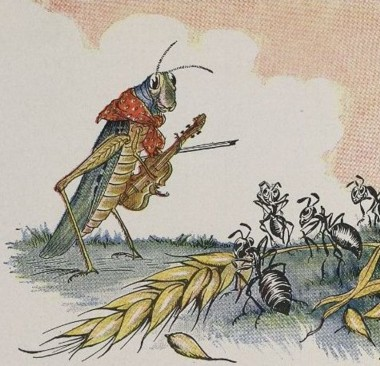
\includegraphics[width=1\textwidth]{ant-grashopper}
	\caption[Ant and Grashopper]{Ant and Grasshopper, Illustration by Milo Winter from 1919 (1888-1956)}
	\begin{flushleft}
		\scriptsize{\citeauthor{Aesop}'s (\citeyear{Aesop} BC) ``Ant and the Grasshopper'', illustrated by Milo Winter (1888-1956) in 1919.
Originally uploaded by \href{http://www.gutenberg.org/etext/19994}{Project Gutenberg}, via \href{http://commons.wikimedia.org/wiki/File:The-Ant-and-the-Grasshopper---Project-Gutenberg-etext-19994.jpg}{Wikimedia}}.
	\end{flushleft}
\end{figure}

It really is a fabled tax.

\subparagraph{History}
%last discussed, suggested in 2005 by Bush's tax reform group http://www.economist.com/node/5061687
%also get into the reasons why the USA tax failed.

\paragraph{Expenditure Tax (ET)}
	\phantomsection
	\label{sec:ET}
%must write this, it's simple
%I also think this is the evil twin!
%it is NOT cash-flow based!

%random ideas, edits, additions for thesis
%[ ] to bash FairTax.org (evil twins):
%http://www.taxpolicycenter.org/publications/urlprint.cfm?ID=901139
	%[ ] good source (popular) for the positional consumption race and its efficiency losses:
%http://prospect.org/cs/articles?article=postconsumer-prosperity#
	%[ ] really bash the Bradford X-Tax for good:
%It has limited progression (0-35% on the labor component, 25% on the non-labor VAT).
%This isn't exactly very good progression.
%Also, it falls only on labor.
%It's not a progressive consumption tax.
%It's a VAT with some poor relief.

\subsection{Taxes on Wealth} %substanzsteuer

\subsubsection{Taxes on Unimproved Nature}

%see diverse notes on google docs re:
%Dahrendorf krams

\paragraph{Land Value Tax (LVT)}
	\phantomsection
	\label{sec:LVT}
%needs to be written

%note about the LVT:
%it HAS limited income;
%it cannot be taxed beyond rental value people would simply stop using land at all (because the supply curve is completely inelastic).
	%so you might need other taxes, too.
	%it's not clear how much value add comes from this one factor

%include the LVT in the circular flow diagram, together with other rents

%note that the LVT requires some difficult evaluations;
%it may cause some of the same illiqudity and other market reactions that we already now.
	%notably, market evaluations for untraded land (for example, in the insurance business and/or for mortgages) will not help much, because these are in turn, market interactions that may be distorted, or equivalently, cause their own DWLs.
	%modern algorithms and data mining might help a little, in so far that land is comparable, which seems possible (it doesn't have sharp gradients).
	%alternatively, auctioning off land periodically might be the better solution to this problem -- it would have the same distributive effects (NO land rent), but may be politically difficult.
		%unclear if you can get the same steering effects on land concentration

%normative attractiveness:
%no one actually created land, it is but a by-product of capturing, or at one point, having captured, parts of land.

%there is a problem of transitional justice;
%people who have now invested in land, as opposed to other assets, may be at a disadvantage (or will they?)
	%if you have land, you're taxed on the unimproved value, if the rental value is lower, you don't use the land, so land use get's smaller, some land is abandoned (but it'll stop generating revenue at that point)
	%solow also says this:
%‘Theoretical’’ is an essential qualifier here, because consensus evaporates once the papers turn to real-world implementation issues.
%One such issue is emphasized by discussant Robert Solow (p.
%278):
%high tax rates on land values would mean departing dramatically from existing tax policy, with correspondingly dramatic capital losses:
%‘‘Expropriating land values today would have no semblance of fairness.
%Suppose I have just paid through the nose for a prime beach lot.
%I have no unearned increment from the land.
%If you now tax away the rent, you are in effect taxing away the savings that enabled me to buy it.
%The original appropriator of the land is long gone.’’ /this is via \cite{Tomlinson2001}


%— Adam Smith , The Wealth of Nations, Book V, Chapter 2, Article I:
%Taxes upon the Rent of Houses:
	%Ground-rents are a still more proper subject of taxation than the rent of houses.
%A tax upon ground-rents would not raise the rents of houses.
%It would fall altogether upon the owner of the ground-rent, who acts always as a monopolist, and exacts the greatest rent which can be got for the use of his ground.
%More or less can be got for it according as the competitors happen to be richer or poorer, or can afford to gratify their fancy for a particular spot of ground at a greater or smaller expense.
%In every country the greatest number of rich competitors is in the capital, and it is there accordingly that the highest ground-rents are always to be found.
%As the wealth of those competitors would in no respect be increased by a tax upon ground-rents, they would not probably be disposed to pay more for the use of the ground.
%Whether the tax was to be advanced by the inhabitant, or by the owner of the ground, would be of little importance.
%The more the inhabitant was obliged to pay for the tax, the less he would incline to pay for the ground;
%so that the final payment of the tax would fall altogether upon the owner of the ground-rent.

%note neutrality of the tax

%Paul Samuelson:
%Paul Samuelson strongly supported a land value tax.
%"Our ideal society finds it essential to put a rent on land as a way of maximizing the total consumption available to the society.
%\ldotsPure land rent is in the nature of a 'surplus' which can be taxed heavily without distorting production incentives or efficiency.
%A land value tax can be called 'the useful tax on measured land surplus'." (wikipedia)

%Friedman from Wikipedia:
%Milton Friedman stated:
%"There's a sense in which all taxes are antagonistic to free enterprise -- and yet we need taxes.
%\ldotsSo the question is, which are the least bad taxes?
%In my opinion the least bad tax is the property tax on the unimproved value of land, the Henry George argument of many, many years ago."

%Krugman from Wikipedia:
%Paul Krugman agrees that a land value tax is efficient, however he disputes whether it should be considered a single tax, as he believes it would not be enough alone, excluding taxes on natural resource rents and other Georgistesque taxes, to fund a welfare state.
%"Believe it or not, urban economics models actually do suggest that Georgist taxation would be the right approach at least to finance city growth.
%But I would just say:
%I don’t think you can raise nearly enough money to run a modern welfare state by taxing land [only].” http://www.psmag.com/politics/this-land-is-your-land-3392/

%The Nobelist Joseph Stiglitz writes "Not only was Henry George correct that a tax on land is non-distortionary, but in an equilibrium society \ldots
%tax on land raises just enough revenue to finance the (optimally chosen) level of government expenditure.

%\cite{Tomlinson2001}
	%Book reviews / Regional Science and Urban Economics 31 ( 2001 ) 601 – 641 635
 %properties that sell are developed properties.
%Reschovsky’s concluding comment (p.
%234) underscores the issue’s significance:
%‘‘In my view, the most important unresolved issue concerning the adoption of a land value tax by a city or state government is the ability of that city or state to provide high-quality land value assessments that will be widely accepted by taxpayers, and will reflect as closely as possible the ‘highest and best use’ of each parcel of land.
%Experts clearly disagree about the feasibility of assessing land values.
%One way to resolve this issue would be for at least one state to attempt to implement a serious state-wide assessment of land values.
%This in turn would allow for full evaluation of the land value tax in a state or local government setting.’


\subparagraph{Pigouvian Element.} %comment on its pigouvian element,

\subparagraph{Other Natural Resources}
%\ldots
%but NOT CO2E, it does not replace that, it only deals with the inequality AND a little bit the commons problem of resources
%when applied to other material resources, too, the LVT becomes a, or might replace severance taxes.

%also compare this to auctioning off.
%The same could be done for land, except that would require land reform, so maybe the LVT is the smarter choice.

%notice that this unlikely to hit farmers (as they might expect) and other marginal uses of land.

%also notice the foundational beauty of this (smith mentions it):
%it's about taxing that part of your property that is valuable because of the stuff that other people around it (and public infrastructure) are doing.
%It's so beautiful.

\subsubsection{Taxes on Property}

\paragraph{Property Tax}
	\phantomsection
	\label{sec:PT}
%note use in the US for local school finance
%only on real estate, but could be other stuff

\paragraph{Stamp Duty}
	\phantomsection
	\label{sec:SD}

\subsubsection{Taxes on Net Worth}

\paragraph{Wealth Tax (WT)}
	\phantomsection
	\label{sec:WT}
The Wealth Tax is a tax on the net wealth ($assets$ $-$ $liabilities$) of natural persons.
It requires a balance sheet account for all tax liable individuals, including some method of valuation for \hyperref[des:liquid-assets]{illiquid assets}.
Wealth Taxes are typically progressive in schedule.
They are levied only in a few OECD countries, including France (up to 1.8\% p.a.) and Switzerland (up to 1.5\% p.a.).

%Include the estate and gift taxes as a subclass of taxes on net worth, because these are just triggered at a particular point in time (death).
%They are, crucial and by definition, not income taxes because they are not LINKED TO ANY EXCHANGE, for if they were, they would be incomes.
%Also note this in the definition of incomes:
%they are exchange incomes, not gifts.
	%or are they?
%maybe I need to include gift and estate taxes somewhere \ldots

%mention subsets Property Tax \gls{pt} and Stamp Duty \gls{wt} here.
%Also refer to \gls{lvt}

\subsection{Non-Taxes}

\paragraph{Financial Transaction Tax (FTT)}
	\phantomsection
	\label{sec:FTT}
%need to write this

\paragraph{ecotax}
	\phantomsection
	\label{sec:Ecotax}
%need to write this
%note that this is not actually a tax in germany, but just a bunch of changes in different quantity taxes on energy.

\paragraph{Negative Income Tax (NIT)}
	\phantomsection
	\label{sec:NIT}
The Negative Income Tax (NIT) is a subsidy for low wage earners, not a tax.
It does not raise, but spends revenue.
It is included here because of its broad redistributive impact and its technical implementation as a ``tax''.

The NIT was suggested by Milton \cite{Friedman1962} as an elegant replacement for minimum wage legislation and \hyperref[sec:StructuralUnemployment]{broadly equivalent} (page \pageref{sec:StructuralUnemployment}) social security transfers.
Under the NIT, workers would receive progressive transfer payments for hourly market wages below the socially acceptable minimum.
However, in contrast to current income supplements, real market wage increases are not entirely eaten up by transfer cuts:
at any given level of income, earning more on the market will leave you with more net in the bank.
For example, under a minimum acceptable hourly income of \euro{}7.50 (current minimum wage proposal in Germany), moving from a \euro{}2.00 market price to a \euro{}4.00 market price job could increase your post-tax income from \euro{}7.50 (transfer \euro{}5.50) to \euro{}8.50 (transfer \euro{}4.50), always maintaining your incentives to earn more on the market.
This may also help to counteract rent-seeking exploitation by low-paying firms.

\section{The Contest}
	\label{sec:contest}
I now compare the merits of the above taxes according to the desiderata established so far.
It will not be necessary to score every individual tax.
Instead, they can be grouped in families of taxes all performing roughly equivalently in terms of the desiderata relevant here.

Results are summarized in \autoref{sec:Scores}.

May the perfect tax win.

\subsection[Indirect, Proportional Taxes]{The Forerunner:\ Indirect, Proportional Taxes:\ VAT \& Payroll}
	\label{sec:ScoreVAT}
Indirect, proportional taxes are the forerunners in tax choice today.
For the last two to three decades, they have assumed an ever greater share of GDP, compared to other taxes (for Germany and the UK, see \citep[11]{Kemmerling2009}.

VAT and Payroll, for all their differences, share key characteristics:
they are indirect, they are proportional and they fall on relatively immobile bases.
 %and therefore, Payroll, at least, is regressive

\paragraph{Neutrality.}
The key merit of indirect, proportional taxation is its neutrality to relative prices in the economy:
deadweight losses are indeed \hyperref[des:minimal-DWL]{minimal}, as per desideratum \ref{des:minimal-DWL}.

\subparagraph{Everyone Has to Consume.}
For the VAT, the neutrality case is clear-cut.
Ultimately, people can only spend the savings and (capital, labor) income they have on goods on the market.
If buying of \emph{all} goods is proportionally taxed, people have no way to avoid the tax.
They \emph{cannot} react to a price signal that is \emph{universally} increased:
their \hyperref[eq:PED]{price elasticity of demand} (page \pageref{eq:PED}) is minimal.
The same holds for sellers:
they have to sell to someone.
When every potential buyer has to bear the same tax, sellers have no way to react.
Their \hyperref[eq:PES]{price elasticity of supply} (p.~\pageref{eq:PES}) is minimal, too.
The VAT falls on a \hyperref[des:tax-inelastic]{maximally inelastic base} as per desideratum \ref{des:tax-inelastic}.

\subparagraph{Everyone Has to Work \ldots}
A proportional payroll tax is neutral when one accepts an exclusive, \hyperref[sec:OSN]{ordinary savings norm} (page \pageref{sec:OSN}).
When capital rents are only \emph{compensation} for risky, deferred consumption all savings and capital rents are ultimately labor incomes.
Under the \hyperref[sec:OSN]{ordinary savings norm}, someone living off her savings is someone living off her past work.
In short, to consume and to live at all, everybody has to work, for someone, sometime.
If you have to work for someone, and every potential employment is subject to the same, proportional tax, you cannot react to the tax.
Again, the \hyperref[eq:PES]{price elasticity} of labor supply (page \pageref{eq:PES}) is minimal.
The same holds for employers:
they have to employ someone.
If every potential employer is subjected to the same, proportional tax, their \hyperref[eq:PES]{price elasticity} of labor demand (page \pageref{eq:PES}) is minimal, too.
\footnote{
	In the real world, payroll taxes are levied only on employees, and not on self-employed people.
	That practice \emph{does} change relative prices of employed and self-employed work.
	Analytically, this discrimination is an aberration from a perfect payroll tax.
	In principle, self-employed people should be liable for a payroll tax on the wages they pay themselves.
}
	%scheinselbständige shows how this loophole can be exploited - often to the detriment of the self employed person.

\subparagraph{\ldots Except the Rich.}
Under a \hyperref[sec:Y2C]{yield to capital norm} (page \pageref{sec:Y2C}), a proportional tax is not neutral.
When capital rents are a genuine increment to wealth, there is an alternative to work:
you can either work, or live off your interest.
In formal terms, rich people can substitute their labor income with capital income.
As the availability of substitutes increases price elasticity, the labor supply by rich people is no longer price inelastic.
Absent the payroll tax, they might have elected to work more than they will if their labor income is taxed.
	%this is, at the and, questionable.
%Do people really work more because of pay?
%at which level?
%discuss homo econ.
%Resolution:
%if incentives should matter, to the degree that they do, we should maie it netraul.
%If they are, as I suspect, neglibible/strictly limited, corrects should be small.

\subparagraph{Ideally, A Ordoliberally Hygienic Tax.}
A neutral tax, by definition, has no fee or pigouvian component.
A VAT or payroll tax with a proportional, uniform rate is \hyperref[des:ordoliberal-hygiene]{ordoliberally hygienic} as per desideratum \ref{des:ordoliberal-hygiene}.

\paragraph{Redistribution $=$ General Revenue?}
To the extent that proportional taxation is accepted as an equity norm (!), a VAT or payroll that goes into general government revenue is a proper instrument both to \hyperref[des:redistribution-and-revenue-are-one]{redistribute and to raise revenue}, as a desirable tax should as per desideratum \ref{des:redistribution-and-revenue-are-one}.

In Germany and many other countries, \emph{capped} payroll taxes are used to raise social insurance contributions.
Here, redistribution and revenue generation undesirably interact.

First, social insurance contributions are proper taxes:
	%ref defunct
		% \hyperref[sec:SICAreTaxes]{social insurance contributions are proper taxes} (page \pageref{sec:SICAreTaxes}):
they serve to pool risks and they redistribute between old and young, healthy and sick.
Second, these services are actually provided universally and unconditionally:
as a last resort, the (German) welfare state pays even for those who have \emph{not} contributed.
The welfare state polity, has in other words, already adopted an allocative norm.

Raising revenue for these very services on a \emph{regressive} schedule (capped) on only some incomes (employed labor) embodies another, very specific allocation, for which no normative justification is readily available.
In Germany, only employed people pay for the health insurance of all other employed people.
Exactly \emph{why}, at minimum, self-employed people do not also contribute to this risk pool is unexplained, but allocatively consequential.

\paragraph{Fairness.} At best, a VAT or payroll tax can be regarded as a proportional taxation on \hyperref[des:personal-taxation]{natural persons} as per desideratum \ref{des:personal-taxation}.
\footnote{
	Social insurance contributions as a selective payroll tax on capped labor incomes \emph{do not} fall on all natural persons, but only some.
	Again, an ideal payroll tax would burden everyone.
}
It cannot accommodate progression, let alone an arbitrarily steep schedule.
	%ref defunct
		% \hyperref[des:Progression]{progression}, let alone an \hyperref[des:SharpProgression]{arbitrarily steep schedule} as per  desiderata \ref{des:Progression} and \ref{des:SharpProgression}.

\subparagraph{Payroll:~Regressive.}
An (ideal) payroll tax is proportional only under an \hyperref[sec:OSN]{ordinary savings norm} (page \pageref{sec:OSN}).
When capital rents are regarded as proper income (\hyperref[sec:Y2C]{Yield-to-Capital Norm}, page \pageref{sec:Y2C}), a payroll tax falls only on one of two types of incomes.
A payroll tax is clearly not \hyperref[des:structural-agnosticism]{agnostic towards labor and capital incomes}, as mandated by desideratum \ref{des:structural-agnosticism}.

\subparagraph{VAT:~Proportional.}
No matter the savings norm, a VAT is straightforwardly proportional, because \emph{all} income is ultimately consumed and tax liable to generate utility.
	%include argument, table, example here

\subparagraph{Different Rates Are Not An Option.}
One common alteration to make the VAT fairer is to adopt different rates for different types of products.
Goods that cover basic needs (food) often enjoy a lower VAT rate.
In a complex economy and modern society, it is impossible to easily determine which goods satisfy basic needs and which do not.
Is a meat a basic need?
Is a filet mignon?
Is a filet mignon every day?
%more generally, this violates the norm of neutrality, it will affect less people who buy 10 sedans than people who buy 1 luxury car.
%This is about as non-agnostic as it gets.

When the state \emph{does} establish different VAT rates, it risks becoming a micro-manager of fairness and will create arbitrary incentives for cross-substitution.
	%&also, there are loopholes for fraud!

\paragraph{The Problems of Proportional Taxation.}
Aside from not being progressive, a proportional tax raises a number of \hyperref[sec:tax-optimality]{efficiency} problems (page \pageref{sec:tax-optimality}).

\subparagraph{Diminishing Utility and Positional Consumption.}
As proportional taxes, VAT and payroll cannot consider \hyperref[sec:diminishing-marginal-utility]{diminishing marginal utility} of wealth, income or consumption.
	%ref defunct
		% as demanded by desideratum \ref{des:DiminishingUtility}.
Whether you are struggling to pay for the first class trip of your child or whether you are thinking about signing up your child for the third summer school, the taxman will treat these two transactions equally, irrespective of the clearly differential impact on the subjective well-being --- not to mention opportunity --- of parents and child in these two families.

Similarly, a proportional VAT on consumption can also not curb \hyperref[sec:positional-race]{positional races} (\autopageref{sec:positional-race}).
	%ref defunct
	% as mandated in desideratum \ref{des:ConspicuousConsumption}.
Whether you are buying a high-priced Mercedes sedan because you enjoy a luxury car during your frequent trips on the German autobahn, or whether you are buying it merely because you do not want the smaller car than your neighbor, the taxman will treat these two transactions equally, with no regard to a potentially wasteful, positional component of consumption.

\subparagraph{Proportional Taxation Raises the Effective Price Floor of Labor.}
	\phantomsection
	\label{sec:PropTaxDWL}
Most problematically, any proportional taxation will make it relatively more expensive for low-income earners to make ends meet.
In welfare states with legislated or effective minimal standards of living, such an increase in the real costs of living will push more people into structural unemployment.
When every trip to the grocery store gets more expensive, more low-skilled people will be unable to afford a socially acceptable minimal standard of living from their equilibrium incomes.
Conversely, the (very price-elastic) demand for such low-qualification service jobs drops dramatically, as struggling workers try to extract higher wages (Scharpf in foreword to \citealt[12ff]{Ganghof2004}).
An equivalent dynamic holds for proportional payroll taxes.

Proportional taxation raises the \hyperref[des:low-price-floor]{effective price floor for low-productivity labor} in violation of desideratum \ref{des:low-price-floor}.
Present some income-replacing transfer scheme, as is nearly universally the case in developed welfare states, supply for low-productivity work becomes very elastic:
you can either work for \emph{less} net purchasing power, or receive \emph{same} or a little more from the state for not working at all.
Proportional VAT or payroll taxation then creates a substantial \hyperref[des:minimal-DWL]{dwl} of structural unemployment, disallowed in desideratum \ref{des:minimal-DWL}.
\footnote{
	This is \emph{not} some kind of welfare-mother argument.
	It is not that lazy people cause structural unemployment and free-ride on the polity.
	Rather, the polity makes it systematically impossible for some of its members to participate gainfully in the economy.
}
		%gainfully and dethly?
		%add a neoliberal source that argues for natural unemployment here.

\subparagraph{Limited Stabilization.}
Proportional taxation, by definition cannot serve as an automatic stabilizer.
	% \hyperref[des:AutomaticStabilizer]{automatic stabilizer}, as demanded by desideratum
	%ref missing. \ref{des:AutomaticStabilizer}.
When the schedule is linear, it does not matter how lumpy your consumption is.
A VAT or ideal payroll will do nothing to prevent you from buying nothing during a bust, and too much during a boom.

A proportional VAT could, theoretically serve as an discretionary stabilizer if government were to lower the VAT rate during the downturn.
	%ref defunct
	% \hyperref[des:DiscretionaryStabilizer]{discretionary stabilizer}
People would have an incentive to buy at lower taxes during the downturn, rather than later at higher rates.

Unemployment insurance works as an automatic stabilizer because of how the revenue is \emph{used}, and not how it is \emph{raised}.
Consumption is smoothed out as the incomes of laid-off workers are insured in the medium term.
Two problems remain:
First, laid-off workers can still consume less than they optimally should, maybe because they are anticipating a prolonged, uninsured downturn.
Second, unemployment insurance would be a much better automatic stabilizer if it were raised in a manner that also smoothes consumption.

\paragraph{A Mixed Bag For Capitalism.}
On the pro side, a VAT and proportional payroll tax let entrepreneurs make their own production decisions, and on their own dime and incentive.
	% \hyperref[des:Entrepreneurship]{entrepreneurs make their own production decisions}, and on their own dime and incentive.
	% \hyperref[des:Incentives]{dime and incentive}.
	%refs broken.
		% as mandated in desiderata \ref{des:Entrepreneurship} and \ref{des:Incentives}.

A VAT and proportional payroll tax also do not require \hyperref[des:liquid-assets]{evaluation of illiquid assets}, as disallowed by desideratum \ref{des:liquid-assets}.

On the other hand, a VAT and proportional payroll tax does little to avoid \hyperref[sec:inequality-dynamics]{runaway capital accumulation} (page \pageref{sec:inequality-dynamics}ff.).
If capital is concentrated in the hands of only a few people, the rest will not be able to close intelligently incentivized deals on their unobservable effort and uncertain innovations.
	%href missing broad ownership
	%Tightly concentrated capital is in violation of desideratum \ref{des:BroadOwnership}.

\paragraph{A Tiny Little Bit Difference Principle.}
For all its equity and efficiency shortcomings, a proportional VAT shares the fundamental merit of all consumption taxes:
it taxes a normatively justifiable basis.
Taxing consumption, not incomes, may be desirable under the the \hyperref[des:difference-principle]{difference principle}, as per desideratum \ref{des:difference-principle}.
This \hyperref[sec:foundational-beauty]{foundational argument} is presented in greater detail and strength in \ref{sec:foundational-beauty} on the \emph{Progressive} Consumption Tax.
Absent progression, the difference principle merits of the VAT are negligible.

The merit of consumption taxation under VAT also manifests itself in the (somewhat
\footnote{
	Only a PCT, by virtue of its progressive schedule, will \hyperref[sec:ScorePCT]{allow for a truly \emph{arbitrary} savings rate} as argued in \autoref{sec:ScorePCT}.
}
positive savings rate it allows for..
	%ref broken
	%\hyperref[des:Savings]{positive savings rate} it allows for, as mandated in desideratum \ref{des:Savings}.
If government would raise its revenue exclusively through a VAT, people's incentive to save would be unaltered:
as argued in the above, a VAT is agnostic towards capital or labor incomes.

\subsection[Direct, Progressive Taxes]{The Old Hand ---\\Direct, Progressive Taxes:~PIT, CIT \& Dual PIT}
	\label{sec:ScorePIT}
The \gls{pit} is the archetypical modern tax designed to redistribute.
It was conceived in the early to mid 19th century to address the inequities of early capitalism.

\paragraph{Income Taxation Punishes Saving.}
A \gls{pit} can cause two different kinds of \hyperref[des:minimal-DWL]{DWLs disallowed} in desideratum \ref{des:minimal-DWL}.

First, if insufficiently progressive (= near proportional), it causes the \hyperref[sec:PropTaxDWL]{DWL of proportional taxation} discussed for VAT and payroll taxes (page \pageref{sec:PropTaxDWL}).

Second, if it is sufficiently progressive on both labor and capital incomes, it taxes savings twice:
once when they are earned, and a second time when they yield an interest (and yet again when they yield a compound interest).
This has a number of negative implications.

When people can avoid double taxation by consuming income right away, they may very well do so.
Capital incomes are taxed, even though saving is elastic.
This conflicts with desideratum \ref{des:tax-inelastic} (\hyperref[des:tax-inelastic]{tax inelastic bases}).
Things become even more awry when we consider investments (savings) of different risk.
When the (uncertain, but higher) rewards of risky investment are taxed progressively, people will have a smaller incentive to run the risk in the first place.
The PIT still allows for local, decentralized production decisions but incentives are substantially dampened.
 	% ref is broken, used to be for broad ownership and entrepreneurship and incentives in violation of desideratum \ref{des:incentives}.

%broken hrefs
	%Because it taxes savings twice, a PIT is in violation of desideratum \ref{des:Savings} on an \hyperref[des:Savings]{arbitrary savings rate} (page \pageref{des:Savings}) and desideratum \ref{des:structural-agnosticism} on \hyperref[des:structural-agnosticism]{structural agnosticism} (page \pageref{des:structural-agnosticism}).
A PIT discourages saving, and it falls twice on capital income, and only once on labor income.
	%simplyfy language
	%also:
%use income-source agnosticism instead of the other term?

\paragraph{The Merits of Progression.}
%broken refs
%To the extent that a PIT is progressive, it satisfies desiderata \ref{des:DiminishingUtility} on \hyperref[des:DiminishingUtility]{the diminishing marginal utility of income} (page \pageref{des:DiminishingUtility}) and \ref{des:Progression} on \hyperref[des:Progression]{progression} (page \pageref{des:Progression}).
It also serves to \hyperref[des:low-price-floor]{lower the price floor} of labor as per desideratum \ref{des:low-price-floor}.
The problematic double taxation of capital incomes also serves to substantially dampen \hyperref[sec:inequality-dynamics]{runaway capital accumulation} and ensures \emph{some} degree of broad ownership.
%broken ref
	% \hyperref[des:BroadOwnership]{broad ownership} as mandated in desideratum \ref{des:BroadOwnership} \citep[810]{McCaffery2005}.
	%degree of ownershiop depends on the spending side, too, of course.
%Explain this

\paragraph{The Limits of Progression Under the PIT.}
A tax on \emph{income}, by definition, does little to curb \hyperref[sec:positional-race]{positional races}.
	% as mandated in desideratum \ref{des:ConspicuousConsumption}.

More fundamentally, a PIT does \emph{not} allow for truly arbitrarily steep schedules.
	% \hyperref[des:SharpProgression]{arbitrarily steep schedule} as per desideratum \ref{des:SharpProgression}.
	%actually, this is horeshit; no tax does -- talk about tradeoffs
	%great econ quote (who said this?) In economics there are no solutions, only tradeoffs.
For a high \emph{average} tax rate on incomes say, 50\%, \emph{marginal} tax rates would be prohibitively high.
Such high marginal tax rates would all but destroy \hyperref[des:Incentives]{incentives to invest} at that margin at all.
	%, violating desiderata \ref{des:Incentives}, \ref{des:Savings}, \ref{des:minimal-DWL} and \ref{des:tax-inelastic}.
It seems likely that a PIT will be no match to the \hyperref[sec:inequality-dynamics]{governing dynamics of self-reinforcing inequality} (page \pageref{sec:inequality-dynamics}), given its limited steepness in progression.
	%again, via coinsumption, it also applies to the PCT:
%Or it doesnt because compount interest?

\paragraph{No Stabilization.}
As any tax on income, the PIT cannot serve as an effective automatic or discretionary stabilizer.
	% \hyperref[des:AutomaticStabilizer]{automatic stabilizer}, or \hyperref[des:DiscretionaryStabilizer]{discretionary stabilizer} as demanded in desiderata \ref{des:AutomaticStabilizer} and \ref{des:DiscretionaryStabilizer}.

\paragraph{The Systemic Flaws of the PIT.}
Aside from its limited and problematic merits, the PIT carries with it some unavoidable, inherent flaws.

\subparagraph{The PIT's Ugly or Unfair trade-off:~Accrual vs.~Realization.}
Because the PIT is based on flows of economic welfare, it requires a method to measure these flows.
Whenever assets are illiquid
	% \hyperref[sec:Illiquid]{illiquid} (page \pageref{sec:Illiquid}),
the taxman can either wait indefinitely for realization, or tax on some assumed accrual.
Either way, substantial welfare losses ensue and desideratum \ref{des:liquid-assets} on the \hyperref[des:liquid-assets]{minimal taxation of illiquid assets} is violated.
	%pct requires balance sheet accounting!
%not just cash-flow!

Income taxation on accrual or realization also has substantial equity implications.
In contrast to the VAT, it is \emph{not} merely a matter of timing when we pay the income tax.

\begin{quote}
	``Such a statement reveals a basic failure to understand --- or a desire that others not understand --- the nature of income taxation and tax avoidance:
	[\ldots] if income tax can be postponed [\ldots], interest (or other capital income) can be earned on a tax deferred basis in the meantime.''
	\\*
	--- McLure (1988 \citealt[as cited in][125]{Seidman1997})
	%find complete reference
	%twitter this!
\end{quote}

In short:
taxation on realization ignores compound interest.

\subparagraph{Tax Evasion 101:~Buy, Borrow, Die.}
	\phantomsection
	\label{sec:TaxEvasion101}
A sinister exploitation of the evaluation problem of the PIT goes by the name of \emph{buy, borrow, die}.
\footnote{
	I take these lessons in ``tax planning 101'' --- only slightly tongue in cheek --- from \citeauthor{McCaffery2005}'s seminal piece on \emph{A New Understanding of Tax} \citeyearpar[888ff]{McCaffery2005}.
}

It emerges from the following three doctrines, all of which make sense in isolation.

%McCaffery:
	%taxes have become voluntary.Read more at location 57   • Delete this highlight
	%Add a note

First, a PIT never taxes debt as income.
It makes little sense to tax debt:
according to \citeauthor{Haig1921}-\citeauthor{Simons1938} (equation {eq:HaigSimons}) and common intuition, the income-generating ability of a person does not change just because she takes out a loan.
Consequently, people pay their taxes on the income they use to repay principal and interest.

Second, for the practical reason of avoiding evaluations by a central planner, the PIT is levied on realization, not accrual.

Third, for \citeauthor{Haig1921}-\citeauthor{Simons1938} and common intuition, heirs are (estate) taxed only net of assets and liabilities handed down to them.

So far so good?
These three trivially intuitive doctrines, in combination constitute the fatal achilles heel of effective capital income taxation.
Tax evaders can follow a simple, and entirely legal strategy.
First, they \emph{buy} appreciating, but illiquid assets.
In a second step, they \emph{borrow} money on the appreciating asset as collateral.
Recall that this cash inflow is not taxed.
Also recall that lenders may very well consider the yet-illiquid appreciation of the asset in extending their loan terms.
Tax evaders can now spend out of the appreciation of the asset without paying \emph{any} capital income tax on this de-facto accrual of welfare.
Third, tax evaders \emph{die} and bequest their assets to someone else.
That someone else is liable only for estate tax on the \emph{net} value of the assets and liabilities.
The consumption of the deceased tax evader is deducted from the net value.
Again, ultimately, and irrevocably, consumed capital incomes escape taxation.
	%alternatively, you make inheritors liable for the decades of tax liability and they'll just pass on the inheritance

This loophole, like the underlying problem of \hyperref[sec:flight-2-illiquid]{illiquid assets}, is \emph{not} a practical aberration that could conceivably be closed.
Any income tax on realization will offer this evasive strategy.
%is this an entirely new problem, or does this fall adequately under "don't tax illiquid stuff?" Can I break it down like that?
%Or is there maybe another thing behind it?
%Timing?
%Is it all accrual vs realization?

This is not a hypothetical or esoteric problem.
The pre-2007 housing bubble in the U.S., Spain and elsewhere was --- amongst other factors --- also fueled by this strategy.
Houses were good illiquid assets (\emph{buy}).
Banks willingly offered mortgages on the houses (\emph{borrow}).
They also happily refinanced the loan, if the suggested (but unrealized!) fair market value of the house had increased.
Consumers took out a bigger mortgage on the (supposedly) appreciated house and spent the difference on a new SUV and a flat screen TV.
All tax free.

Appreciation in illiquid assets is no small component of our economic growth.
A colossal share of the real welfare that accrues to capital income earners escapes income taxation without further notice, and any readily available fix.

\subparagraph{The PIT's Ugly Backstops:~The Estate and Gift Tax.}
It follows from the strategy of tax evasion 101 that an estate and gift tax are necessary backstops to the PIT.
Without a tax on the substance bequested, unrealized appreciations on illiquid assets would go entirely untaxed.
With an estate and gift tax, ``only'' the consumed part of unrealized appreciations escapes taxation.
%Note:
%the "pure income tax" maybe a cat-dog (Sartori 1991:
%247).
%It's not an actual category.

The estate and gift taxes are, in themselves ugly beasts.
Just like the PIT, they require an evaluation of a flow of economic welfare in the potential absence of a market equilibrium price of that very flow.
If an entrepreneur bequests her family-owned firm to her daughter, no one can know how much it is worth.
Again, problems in the taxation of illiquid assets ensue.
	% \hyperref[sec:Illiquid]{taxation of illiquid assets} ensue (page \pageref{sec:Illiquid}).

\subparagraph{The PIT's Ugly Backstops:~The CIT.}
	\phantomsection
	\label{sec:ScoreCIT}
A PIT has another, even uglier backstop:
the Corporate Income Tax.
Recall that a PIT is meant to tax all incomes, including interest and compound interest.
With only a PIT, tax evaders would have at their disposal a strategy even simpler than tax evasion 101:
they could place (or retain) their savings in an incorporated firm.
First, tax evaders could spread out their (spiky) income over a longer period of time to play the progressive schedule.
A small, but steady trickle of income is better than a large, lumpy flow under a progressive tax.
Second, and more fundamentally problematic, tax evaders can also retain their initial capital income in the corporation and have it earn a compound interest.
Note that the compound interest is earned on a capital income which, ideally, \emph{should} have been taxed \emph{already}.

To avoid this loophole, a PIT needs a CIT to get at the corporate shelter from the income tax \citep[7]{Genschel2005}.
Also empirically, PIT and CIT rates go hand in hand, between countries and over time, further supporting the intricate, if dysfunctional link between the two \citep[14]{Piatkowski2008}.

The CIT is as bad as the PIT, minus the merits of progressive, personal taxation of the PIT.

First, the CIT has no \hyperref[des:determined-incidence]{well-determined incidence} as demanded in desideratum \ref{des:determined-incidence} \citep[918]{McCaffery2005}.
Corporations are fictions.
If you tax them anyway, you violate desideratum \ref{des:personal-taxation} (\hyperref[des:personal-taxation]{personal taxation}).

Second and related, the CIT knows no progression.
To the extent the the CIT ever reliably fell on capital, it made some sense historically when corporate ownership was a reasonable proxy for the propertied classes.
This is no longer the case.
Many people receive capital incomes \citep[XV]{Grabka2007a}.
The CIT has no way of distinguishing \emph{between} different owners \citep[918]{McCaffery2005}.
Whether a particular Volkswagen share belongs to the life insurance of a single working mother or a stock market tycoon, both are taxed at some uniform corporate income rate .
%the CIT is also not internally progressive.

Third, much like the PIT, the CIT itself is plagued by unavoidable loopholes.
The CIT is very sensitive to international tax rate competition:
if CIT rates differ from country to country, multinational companies can easily shift profits to the country with the lowest rate.
A number of strategies are available to do this, the simplest of which is to charge inflated (deflated) prices in intra-company trade \citep[43ff]{Ganghof2004}.
	%this, in fairness, applies to all prigressive taxes
This loophole cannot be closed as inflation (deflation) of intra-company trade prices cannot be reliably detected.
More fundamentally, ``any national claim to a particular share of [a multinational's] profits is hard to justify on the basis of principle'' \citep[61]{Genschel2005}.
%also explain how they can always calculate themselves to zero, not just with arbitrage.


\paragraph{The Downgraded Upgrade:\ The Dual PIT.}
	\phantomsection
	\label{sec:ScoreDualPIT}
To the extent that a Dual PIT has substantially lower, and proportional rates on capital incomes, it alleviates the PIT's disincentives to save and invest.
	% \hyperref[des:Savings]{save} and \hyperref[des:Incentives]{invest} as per desideratum \ref{des:Savings} and \ref{des:Incentives}.
The Dual PIT is simply another non-\hyperref[des:structural-agnosticism]{agnostic} relative burdening of capital and labor incomes in violation of desideratum \ref{des:structural-agnosticism}.

\subparagraph{A Hollowed-Out PIT.}
The relatively smaller burden on capital is hard to justify on principle.
The largest incomes are, by definition, capital incomes.
\footnote{
	Recall that to have a capital income one first has to have a surplus of unconsumed labor income.
}
Charging capital incomes a lower, proportional rate will greatly depress the overall progressivity of the PIT
	% \hyperref[des:Progression]{progression} of the PIT, in violation of desideratum \ref{des:Progression}.
Progression is limited under the PIT already, but will be even more compressed under a dual rate structure.
	%, in violation of \ref{des:SharpProgression}.

To the extent that more of the tax burden falls on labor, a Dual PIT will also raise the \hyperref[des:low-price-floor]{price floor for low-productivity labor supply}, as disallowed in desideratum \ref{des:low-price-floor}.

The Dual PIT is a PIT only in name.
It hollows out the ideal of universal progression.
%universal progression is an ideal, why?
The lower the rate on capital gets, the more a Dual PIT approximates a (progressive) payroll tax.

\subsection[Business Tax]{The Streaker ---\\Local Business Tax (LBT)}
	\label{sec:ScoreLBT}
A tax on the earnings of local businesses shares all of the disadvantages of the CIT.
	%is the idiom clear enough?
%add picture of a litzer
	%also include the financial transaction tax here

More fundamentally, the LBT is not a proper tax.
It should not need to be discussed here at all.

Local authorities provide different kinds of \hyperref[tab:types-of-goods]{goods} (see \autoref{tab:types-of-goods}).
The \hyperref[sec:fiscal-redistribution]{redistribution}, \hyperref[sec:state-insurance]{risk pools} and \hyperref[sec:public-good]{public goods} it provides should be financed out of general revenue.
	%href broken
		% \hyperref[tab:TaxResponses]{general revenue}, as outlined in \autoref{tab:TaxResponses}.\ref{}
A general revenue tax should fall only on \hyperref[des:personal-taxation]{natural persons} as per desideratum \ref{des:personal-taxation}.

Local authorities also provide \hyperref[sec:common-good]{common goods} such as parks and \hyperref[sec:natural-monopoly]{natural monopolies} such as sewers.
\footnote{
	Sometimes, at the margin of local decisions public goods also become common goods or natural monopolies:
	that extra motorway feeder may be necessary only for a small number of logistically intensive firms (rival consumption) and local government may well negotiate with the interested firms on whether to build the road or not (exclusion).
}
Common good and natural monopolies should be financed out of Pigouvian levies (at marginal cost) and fees (at average cost), respectively.
	% as per \autoref{tab:TaxResponses}.

The LBT sits in the nomansland somewhere between general revenue taxation and Pigouvian levy or fee.
It violates the norm of \hyperref[des:ordoliberal-hygiene]{ordoliberal hygiene} as per desideratum \ref{des:ordoliberal-hygiene}.

To the extent that the LBT is used to finances risk pools, public goods and redistributes, it should not be allowed to differ between municipalities.
If universal education is an allocative goal of the broader, national polity, everyone should pay for it.
If fire protection is a public good, everyone should pay for it.
LBT revenue used to finance these things should be replaced by transfers from higher levels of government.
%to avoid arbitrage
	%reference fiscal federalism

To the extent that the LBT is used to finance common goods or natural monopolies, it must specifically fall (at marginal or average cost, respectively) on the very consumption of these goods, and not on the earnings of a firm in general.
If industry pollutes a local river, \emph{every unit of discharged pollution} should be (Pigouvian) taxed at marginal cost, not every firm in the city based on their earnings.
If some firms or citizens in a rural municipality require high-speed internet access (a natural monopoly), each \emph{user} of the network should pay at average costs, not every firm in the vicinity.
%add:
%sometimes, such break-downs might be impractical, in that case, paying it out of general revenue might just be the better ticket.
Also note that LVT can replace this purpose to some extent.

In short, the LBT is an anti-ordoliberal streaker that should never have entered this game of perfect taxation.
It should be marshaled off the playing field as soon as possible.

\subsection{Impotent Redistribution}

\begin{quote}
	\emph{``Advocates of redistributive taxes must wake up and realize that their end is in jeopardy on account of their poor choice of means:
	they are fighting, and losing, the wrong war.''}
	\\*
	--- Edward J.\ \citet[848]{McCaffery2005}
	%add correct citation
\end{quote}


\subsection[Progressive Consumption Tax]{The Dark Horse:~Progressive Consumption Tax (PCT)}
	\label{sec:ScorePCT}

%   * step back carefully from my assumptions:
%even if you don't agree with the politics (redistributive and axiomatic in terms of positional spending) of the pct, you've gotta agree with the efficiency.
%   * even if you don't agree with the PCT, you've gotta agree with the questions it poses.

%add a chapter on the failed USA tax, and the charge that it was too complex.

%Note that what Ganghof + Scharpf 2004:
%37 is incorrect in their treatment of capital incomes.
%They are actually taxed, when they are consumed, given that the tax is cash-flow based (dissavings count!).
%Consider the Haig-Simons.
	%This is a widespread misunderstanding of the PCT, particularly with regards to its evil twins.
	%Contact Ganghof + Scharpf about this mistake!

% Fundamental agreement on the likely advantages of a PCT regime has been reached in the (albeit heterodox) economics literature (conceptually Brümmerhoff 1990:
%357ff, empirically Tomer et al.
%2008, normatively McCaffery 2002).

%What Is The Perfect Tax?
%Friedman is actually a fan of the PCT, and has argued to use it to pay for the war effort in the past.
%This is via Robert Frank 2011 (Darwin).

\paragraph{It's Win-Win-Win-Win:~No DWL Or No DWL \& Less Waste Or Diminishing Marginal Utility.}
	\phantomsection
	\label{sec:WinWin}
The DWL case for the PCT is not clear, but either way, it's good.

Just in \emph{which} way the PCT is good depends on the \hyperref[eq:PED]{price elasticity of demand} in excessive and positional consumption.
	%simplify the language

%let's be honest about this, the DWL case of a PCT is not so clear-cut.
%It might still disincentivize people, because at the end of the day, they get to enjoy less, although, only to the extent that there is actually no race.
%Also, note, that the PCT still does not tax compound interest.
%from \cite{ZimmFina2009}
	%   * Read p.
% 138-159
	%   * feature the Economic cycle page 139 in my thesis, argue why it makes more sense to tax consumption
	%   * 156:
%"Überschreitet die [Einkommens]Besteuerung jedoch ein gewisses Ausmaß, so ist zu erwarten, dass sich negative Auswirkungen auf Investitions- und Arbeitsbereitschaft ergeben und damit das Wachstum beeinträchtig wird.
%Dagegen könnte eingewandt werden, dass ein höherer Anteil der Einkommenssteuer bei gleichem Gesamtsteueraufkommen die Gesamtbelastung nicht verändert, sonder nur wahrnehmbarer macht, weil die Einkommenssteuer für die Besteuerten merklicher ist als die Verbrauchssteuer.
%Für die Wirkung auf Investition und Arbeitsbereitschaft ist aber wahrscheinlich nicht die tatsächliche Belastung eines privaten Haushalts oder Unternehmens entscheidend, sondern nur der Teil der Belastung, der wahrgenommen wird und in die ökonomischen Entscheidungen eingeht."
	%      * Bingo.
%This is the argument for the PCT vs PIT in terms of incentives.

%\cite{MusgPubl1976}
	%   * the PCT "is still a new and exciting idea" (315)
	%   * "In some respects, the approach would be simpler than under the income tax.
%The dilemma of how to deal with unrealized capital gains would disappear.
%If assets were sold, the proceeds would enter into the tax base unless offset by purchases of other assets or an increase in balances.
%Also, there would be no need to determine corporate profits.
%Dividends would appear as receipts and unrealized capital gains obtained through retention of profits or otherwise would be irrelevant until realization occurred and the proceeds were channeled into consumption.
%The difficult problem of depreciation accounting, similarly, would disappear." (316)
	   %   * bingo, bingo, bingo
	%   * "(\ldots) distributional objectives might be achieved with less disincentive effects" (317)
	%   * Contras, needed (316)
	%      * complete recording of cash balances (OK)
	%      * inclusion of imputed consumption (homegrown foods, housing) (OK)
	%      * Borrowing must be acccounted for (indeed, OK)
	%         * "Where the lender was an individual, also subject to tax, he would see to it that this was done so as to reduce his own base;
%but where lending was by institutions not subject to the expenditure tax, lenders would have to be required to file information returns on loans made" (316)
	%         * (OK, this can be done by simply legislating that loans without such reporting are gifts.
	%      * consumer durables (OK)
	%      * "The expense-account problem, difficult enough under the income tax, would assume large proportions" (fringe benefits, acknowlegded)
	%      * education "would pose a similar problem, as they again involve both consumption and investment aspects" (OK)
	%   * "on balance, the administrative diffculties for an expenditure tax may well equal or outweigh those of an income tax.
%For higher-income individuals at least, more or less complete balance-sheet accounting would be needed.
%Yet, this is precisely the income range over which effective administration would matter most.
%At low levels of income, there is relatively little difference between an income and an expenditure tax approach.
%The distinctuon becomes of major importance only as we move up the income scale and the savings rate rises" (317)
	%      * yes, yes, yes, but I don't agree that you need balance-sheet accounting.
%Cash-flow suffices.
%%or do you?
%Actually you need balance-sheet accounting either way for personal progression.

Without further empirical research, they cannot be known.
The PCT will have \emph{very} high marginal rates, possibly well above 100 \%.
Because universal, stark price hikes in the markets for excessive consumption have never occurred, we have no systematic observations regarding the responsiveness of excessive buyers to such price changes.

So what are the alternative outcomes?

\subparagraph{What If:~People Still Consume Excessively.}
If people \emph{do not} respond to the post-tax price hike in excessive consumption, the PCT will tax an \hyperref[des:tax-inelastic]{inelastic base}.
The DWL will be \hyperref[des:minimal-DWL]{minimal}, as per desiderata \ref{des:tax-inelastic} and \ref{des:minimal-DWL}.
Most of what consumers no longer enjoy in excessive consumption will be recouped as government revenue, as illustrated in \autoref{fig:different-incidence}.

Producers will be perfectly elastic in their supply.
At least in the long run,
\footnote{
	This of course depends on a very gentle phasing in of the tax so as to allow producers to cheaply exit their production of excessive consumer goods, and cheaply enter another market.
	This requirement for the \hyperref[sec:Implementation]{implementation} of the PCT is further discussed in \autoref{sec:Implementation}.
}
all producers can shift their production to less expensive consumer goods, or, as described later, to investment goods.
The burden of the PCT will fall exclusively the \hyperref[des:personal-taxation]{natural persons} who ultimately consume goods, as mandated in desideratum \ref{des:personal-taxation}.

\subparagraph{What If:~People Consume Less (Expensive) Things.}
If people \emph{do} respond to the post-tax price hike in excessive consumption, the PCT gains a Pigouvian component, but one that works.
When people consume excessively, they pay for the negative externality of defection in the \hyperref[tab:pd-positional]{Prisoner's Dilemma of positional consumption} (page \pageref{tab:pd-positional}).
Recall that when the Joneses buy a BMW (defect) instead of a VW (cooperation), the utility enjoyed by the VW-owning Does decreases:
they cannot stand having the cheaper car.
Under the PCT, the Joneses pay (dearly) for showing off their BMW.
If their demand for BMWs is price elastic, they may buy the same VW as the Does.

%\begin{table}
%		\caption{The Battle of the Sexes}
%		\label{tab:BoS}
%		\begin{center}
%		\begin{tabular}{m{1cm}m{2,3cm}m{2,3cm}m{2,3cm}m{2,3cm}}
%			& & \multicolumn{2}{c}{\emph{Man}} \\
%			& &Opera & Football\\
%			\cline{3-4}
%			\multicolumn{1}{c}{\multirow{4}{*}{\emph{Women}}} & \multirow{2}{2,3cm}{Opera} & 		\multicolumn{1}{|r|}{2} & \multicolumn{1}{r|}{0}\\
%			\multicolumn{1}{c}{} & \multicolumn{1}{c}{}& \multicolumn{1}{|l|}{3} & \multicolumn{1}{l|}{0}\\
%			\cline{3-4}
%			\multicolumn{1}{c}{} & \multirow{2}{2,3cm}{Football} & \multicolumn{1}{|r|}{0} & \multicolumn{1}{r|}{3}\\
%			\multicolumn{1}{c}{} & \multicolumn{1}{c}{}& \multicolumn{1}{|l|}{0} & \multicolumn{1}{l|}{2}\\
%			\cline{3-4}
%		\end{tabular}
%		\end{center}
%		\scriptsize{The Joneses and the Does are peers, positional consumers and in the market for a new car.
%Payoffs are the net of cost of car ($VW=0$, $BMW=-5$) and status gain from driving the \emph{relatively} more expensive car ($+10$ for superior, $-10$ for inferior, else $0$).
%Larger payoffs are better.\\
%		Prices of the BMWs are inflated so as to include the societal costs of wasteful consumption, here, as in an ideal world, accruing only to the buyer.}
%	\end{table}
%why is this table still in here?

%positional consumption PD is now in mixed economy


Also recall that the level of cooperation in a multiplayer Prisoner's Dilemma is a \hyperref[sec:common-good]{common good} (page \pageref{sec:common-good}).
Contributing to cooperative behavior creates a benefit to other players from which they cannot be \emph{excluded}.
Establishing cooperation is, however, \emph{rival}:
if no one, or too few people cooperate, the benefits of cooperation will not materialize.
Buy buying a VW, the Does contribute to a common-good-like lower level of automobile consumption, from which everyone else can invariably (relatively) benefit.
The Joneses can exploit the thriftiness of the Does by buying a BMW (greater relative utility), or they can partake in the Does thriftiness by buying a cheaper VW (same relative utility, but lower absolute utility), without being looked-down upon by a BMW-owning neighbor.
Either way, the Does cannot prevent the Joneses from benefiting (non-exclusion).
The Joneses buying of a VW is, however rival.
If they end up being the only family on the street that buys the cheaper VW, their triftinness will be inconsequential for everyone else.

Common Goods are best financed out of Pigouvian taxes.
The PCT is that Pigouvian tax of excessive, positional consumption.
It falls on exactly that behavior (excessive consumption) at exactly that price (marginal rate!) which it is meant to discourage.
If rates are sufficiently high and progressive, the PCT can effectively curb  \hyperref[sec:positional-race]{positional races}.
	%, as per desideratum \ref{des:conspicuous-consumption}.
At minimum, it can lower the level of material waste at which positional consumption occurs.

\subparagraph{What If:~People Don't Mind Buying Less (Expensive) Things.}
A Pigouvian tax, by definition, has a DWL.
The DWL of a Pigouvian tax is the very consumer and producer surplus that should never have been realized, because of the social costs hidden to them.

The definition of a DWL assumes that the utility of consumers is accurately measured in their willingness to pay.
Utility and nominal demand curve are the same.
\hyperref[sec:positional-race]{\emph{Positional} consumption} (page \pageref{sec:positional-race})
	%and the \hyperref[sec:PsychicCosts]{psychic costs of stratification} (page \pageref{sec:PsychicCosts})
suggest that people derive utility not from absolute, but relative consumption or status.
People want to have more, or at least not less things and status than other people.

If excessive consumption occurs for positional gain, there \emph{can} be no DWL when that consumption is curtailed for everyone.
No one will be relatively worse off, only less relatively different.
If anything, a more compressed stratification in the material signs of affluence and status will make most of us happier.
	%this is frank

\subparagraph{What If:~People Really Care About Luxury.}
People enjoy having many, and many expensive things not \emph{only} because they want more than their neighbor.
Driving that BMW on the autobahn may be aesthetically pleasing and functionally faster in absolute terms.
\footnote{
	\ldots even though few people will deny that much of autobahn gratification stems from overtaking other cars, if not people.
}

Let's assume for a minute that there really is an absolute, \emph{sheer driving pleasure}
\footnote{
	BMW's claim, \emph{Freude am Fahren}.
}
in driving an expensive car.
Even if there is absolute utility, it is likely to be of marginally decreasing return.
Upgrading from a VW to a BMW will probably bestow more utility on someone than upgrading from a BMW to a Bentley.
By taxing big spenders more, the PCT accounts for \hyperref[sec:diminishing-marginal-utility]{diminishing marginal utility} in excessive consumption.
	%, as demanded by desideratum \ref{des:DiminishingUtility}.
Even in a world of \emph{sheer driving pleasure}, when more people get to upgrade from VW to BMW and fewer from BMW to Bentley, aggregate autophile utility will be maximized.

\paragraph{Sky-High Progression.}
The PCT can be arbitrarily progressive.
	% \hyperref[des:SharpProgression]{arbitrarily progressive}, as prescribed in desideratum \ref{des:SharpProgression}.
For very excessive consumers, rates can be as high as several hundred percent:
literally, the sky is the limit.
Because the PCT falls on consumption, and not on incomes, incentives or entrepreneurship will not be dramatically curtailed.
	% \hyperref[des:Incentives]{incentives} or \hyperref[des:Entpreneurship]{entrepreneurship} will not be dramatically curtailed, as per desiderata \ref{des:Incentives} and \ref{des:Entrepreneurship}.

The ultimate reason for \emph{homo economicus} to work hard and invest wisely is superior consumption.
At first sight, depressed consumption (at higher prices) may appear to reduce incentives.
Consider the trade-offs for \emph{homo economicus} under the PCT:
She can either work an extra hour, or not.
Because she is already very diligent, and likes to \emph{work hard / party (consume) hard}, any additionally enabled unit of consumption will be taxed at a fairly high rate.
At \emph{any} rate of consumption taxation, she will still be better off if she works the extra hour.
	%aha, here we go.
%compare this to incentives under steeply progressive PIT

At the other end of the progressive schedule, rates can be very low or at zero for people who consume very little.
Aside from equity, this also serves to \hyperref[des:low-price-floor]{lower the price floor for low-productivity} labor as per desideratum \ref{des:low-price-floor}.
If the working poor or structurally unemployed pay a zero tax rate on their necessarily minimal consumption, their living standards increase and their reservation wage vis-a-vis the socially acceptable minimum living standard drops.

\paragraph{The PCT Smoothes Consumption.}
Under progressive tax rates on consumption, people are punished for spikes in their consumption.
To have the lowest possible PCT rate for a given level of lifetime consumption, you have to spread out the shopping sprees as evenly as possible.

%frank seems to note somewhere (source unknown, this is from economist web):
	% that the PCT can be counter-cyclical ``If a progressive consumption tax were phased in gradually, its main effect would be to shift spending from consumption to investment, causing productivity and incomes to rise faster.
%Should a recession occur, a temporary cut in consumption taxes would provide a much more powerful stimulus than the traditional temporary cut in income taxes.''

%note that stabilization is always a second best, it'd be nicer if we could fight the cause of busts and booms, but, considering for a moment that we may be unable to do that, such dampers may be a good idea.
%Also, note that if no boom/bust cycle sets in the PCT does not hurt you much.

In a bust or boom, the PCT serves as an automatic stabilizer.
	% elegant \hyperref[des:AutomaticStabilizer]{automatic stabilizer} as per desideratum \ref{des:AutomaticStabilizer}.
Without legislative intervention, people are always incentivized to smooth out their consumption.

The PCT can also serve as a powerful discretionary stabilizer.
	% \hyperref[des:DiscretionaryStabilizer]{discretionary stabilizer} as per desideratum \ref{des:DiscretionaryStabilizer}.
In a bust, legislatures can opt to lower the entire PCT schedule
\footnote{
	In the extreme, government can even make the PCT a variable, progressive subsidy to low-income earners to spend.
	The PCT would then have a negative rate at the very bottom of the schedule:
	government would reward the first units of consumption with a small subsidy once the transaction is done (postpaid).
	Windfall effects would be minimal as people cannot direct the subsidy into further saving.
}
.
For the duration of the bust, people have a greater incentive to consume, knowing that higher rates will return once the economy reverts to its long-term growth path.

The PCT as discretionary stabilizer will be general in impact.
\emph{Whatever} you choose to buy will be cheaper to buy.
Government can inject discretionary stimulus without opening up to clientelist pressures.

The PCT also minimizes windfall effects.
Because you have to consume first to take advantage of the lower rate, you cannot channel the government stimulus into further savings.
In fact, you have to divert from your average consumption path, and consume \emph{more} during the bust.
Just as a \emph{cash-for-clunkers} scheme, the PCT incentivizes people to \emph{dissave}, except for all kinds of consumption and without the waste of clunkers.

\paragraph{Deciding How Much to Consume, and Who Consumes.}
The PCT allows government to set an arbitrary savings rate.
	% \hyperref[des:Savings]{arbitrary savings rate}.
Because it is progressive, the PCT can incentivize saving without \hyperref[des:low-price-floor]{risking working poverty or structural unemployment} (see page \pageref{des:low-price-floor}).
The PCT allows for greater saving than the VAT because it (greatly) incentivizes exactly those people to save more, who can:
the excessive consumers.

\subparagraph{How the PCT Makes You Save More.}
The PCT offers two mechanisms to increase the savings rate.

First, the PCT is simply an elegant revenue stream for government from which it can finance public good projects (public works) or buy investments (sovereign wealth fund).
Both a new (non-congested) motorway and public ownership of some corporation constitute saving.

Second, the PCT is an instrument to alter the save-vs.-consume trade-off for natural persons.
It encourages saving in three distinct ways (the following is from \citep[28ff]{Seidman1997}.
\begin{description}
	\item[The incentive effect]
	of higher post-tax interest rates is more complicated than might appear at first sight.
	Intuitively, tax exempted saving and capital incomes will increase the post-tax interest rates and cause people to save more.
	A \emph{substitution effect} may ensue:
	for every unit of resource saved now, you will receive a greater post-tax payoff in the future.
	You save more.

	On the other hand, a higher post-tax interest rate is an accrual to wealth:
	you just got richer.
	According to the \emph{income effect} of higher interest rates, you may save \emph{less}.
	For fewer units of resources saved now, you will receive a same payoff in the future.
	%I am not sure about my rebuttal of the income effect
	The PCT is less ambiguous in its effects than a change in the market interest rate.
	It has only a substitution effect.
	Because people are (income) taxed before the PCT, too, introducing the PCT does not make them any richer.
	Taxation does not disappear, it merely shifts the base.
	%that's pretty thin, max.
	Think this through again
	\item[The horizontal redistribution (heterogeneity) effect]
	occurs between \emph{equally} affluent persons who differ in how much they consume.
	Consider two millionaires, one of whom spends all his income (affluent consumer), one of whom saves all her income (affluent saver).
	Under income taxation, both pay a (same!) tax on their millionaire income.
	Under the PCT, the affluent saver pays no tax at all, and the (price inelastic) affluent consumer pays twice the income tax for revenues to stay constant.
	The affluent saver gets to save \emph{all} of her income.
	Under income taxation, she can save only the post-tax income.
	In sum, at same public revenues, more money is saved under the PCT than under income taxation.
	\citeauthor{Seidman1997} estimates US savings rates to increase by roughly 11\% due to the heterogeneity effect of a PCT transition.
	\item[The postponement effect]
	occurs as a one-off effect as the tax burden shifts within cohorts from saving at working ages to dissaving during retirement.
	An income tax burdens savings immediately, and early in life once they are earned.
	A PCT burdens savings late in life, when they are consumed.
	At same levels of retirement consumption, people will be able to accumulate more capital earlier.

	To the extent that the postponement effect occurs \emph{within} cohorts, it is a zero-sum intertemporal redistribution between private saving and public revenue.
	It does not, as \citeauthor{Seidman1997} seems to imply, generate genuine new saving in the long term.
	It just postpones government revenue.

	To the extent that the postponement effect occurs \emph{between} cohorts, it can genuinely improve the savings rate \emph{and} public revenue by taxing old savings twice (or even three times).
	The intergenerational equity considerations of this effect are later discussed in \autoref{sec:IntergenerationalIncidence}.
\end{description}

\paragraph{It's not All Pleasure-Delaying.}
So far, the PCT appears to encourage thriftiness over all else.
As Ant --- and even the most die-hard supply-side economist --- will attest, \emph{that} alone would make for a fairly sad state of affairs, with all saving, and ever-delayed consumption.
As Ant learns, the heart wants some music, too.

\subparagraph{The Party's Over.}
As argued in \autoref{sec:long-term-inconsistency}, there are good reasons to believe that we are growing much slower than we could at greater savings, and that, already, we have taken out loans on the future.
No matter what the heart wants, we may have to turn down the music quite a bit.
	%add stuff about carbon-growth link here

\subparagraph{Deciding How Much To Consume.}
Correctly understood, the PCT is actually agnostic towards how much we, as a society, consume or save.
	%, just as the doctor ordered in desideratum \ref{des:Savings}.

What is missing in the description so far --- as it is in much of the politics of tax --- is what happens with the revenue.
Taxation does not reduce resources, but (with a small DWL), merely redirects them.
It is then up to the democratic state, or the individuals to which it redistributes, to decide how much should be saved or invested and how much should be devoted to consumption.

\subparagraph{Deciding Who Consumes.}
Let us (optimistically) assume that the current savings rate is optimal, that aggregate consumption must remain on current levels, and that the public expenditure quota is optimal.
Even in this (unlikely) scenario, the government can use the PCT as a pure redistributive tax to redirect resources from big spenders to small spenders, with no effect on the savings rate or public budgets.
All government would have to do is to either zero-rate the small spenders (a de-facto redistribution \emph{to} them), or hand out additional transfers to them.
To go back to the car example, the PCT would redirect resources from buyers of BMWs to buyers of budget Dacia Logans.

Alternatively, government itself can also spend the revenue on public goods or risk pools.
For instance, government could organize a big parade or a fireworks display on the national holiday.
The savings rate would be unaffected.
The same amount of resources would be spent, just by a different body and for a different purpose.
	%include better example

\subparagraph{S-Classes to Subways.}
Let us now consider what happens when the PCT is used to increase the savings rate, as described in the above.
When implemented with an appropriately \hyperref[sec:GoSlow]{long, gentle transition}, the PCT \emph{does not} lead to a drop in aggregate demand (page \pageref{sec:GoSlow}).
It merely redirects economic resources from the production of consumer goods to the production of capital goods.
Under axiomatically assumed \hyperref[sec:perfect-competition]{perfect competition}, factor markets always clear.
That means that surplus incomes (savings) will always find profitable investment.

%broken ref
%\footnote{
%	At least as long as we are below the exogenously given \hyperref[eq:GoldenRuleSavings]{golden rule of saving} (page \pageref{eq:GoldenRuleSavings}).
%}
This capital deepening of the economy can take many forms.
In the public budget, it can mean building a new school, upgrading our infrastructure, funding basic research or abating and adapting to climate change.
On the marketplace, it can mean building a new factory for solar panels, developing a new biotech patent or building more equity to guard against the next financial crisis.

Whatever the use, in a perfect market, capital deepening is an unambiguously good thing.
It means to enrich our world, with powerful
factories, liberating technologies and empowering education.
When people and institutions are given enough time to adapt to the new incentives, no welfare will be lost and no factors will sit idle.
Mercedes Benz just needs some time to convert its production line from S-Class sedans to economic minivans, or even public transportation.
	%concept:
%let it depreciate!

%note that the LVT may also act as an automatic stabilizer, at least of real estate, because, given the right function, it might curb real estate bubbles.
%problem:
%how do we KNOW the unimproved value of land?!?

\paragraph{The Foundational Beauty of the PCT.}
	\phantomsection
	\label{sec:foundational-beauty}
Gleaming behind its ability to make us all enrich our world, there is a greater normative appeal to the PCT:
its beautiful alignment with a foundational theory of private property.

By taxing consumption, the PCT leaves incentives to work \emph{and} save unaffected.
The PCT \emph{is} \hyperref[des:structural-agnosticism]{agnostic towards labor and capital incomes} as per desideratum \ref{des:structural-agnosticism}.
Like the VAT, it taxes neither of them, but only the component of \emph{all} income that is consumed.
In contrast to the VAT, it does so without sacrificing progression.

``Under the progressive consumption tax'', as industrialist C.
William Hazelett put it to the US Senate in 1939, ``we define income at what it really is.
There is no economic income but the living standard of the taxpayer'' (Hazelett as cited in \citep[15]{Bank2004}.
	%nice quote.

Consumption is the very transaction at which we take a part of the riches of our economy, exclude other people from its partaking and use it up.
The PCT taxes you for \emph{what you take out of the cake}, not for \emph{what you contributed to the cake} \citep[58]{Seidman1997}.

%maybe this stuff has to go to the desirability part?
This foundational ideal of taxation goes back a long time.

Thomas \citeauthor{Hobbes-1651-aa}, in his ``Leviathan'', wrote:

\begin{quotation}
	\emph{``[T]he equality of imposition, consisteth rather in the equality of that which is consumed than of the riches of the persons that consume the same.
	For what reason is there that he which laboureth much, and sparing the fruits of his labour, consumeth little, should be more charged than he that living idlely, getteth little, and spendeth all he gets, seeing the one hath no more protection from the commonwealth than the other?
	But when the impositions are laid upon those things which men consume, every man payeth equally for what he useth, nor is the commonwealth defrauded by the luxurious waste of private men.''}
	\\*
	--- Thomas \citet[386]{Hobbes-1651-aa}
\end{quotation}

Adam \citeauthor{Smith-1776-lq}, in his ``Wealth of a Nation'', wrote:

\begin{quotation}
	\emph{``Every tax ought to be levied at the time, or in the manner, in which it is most likely to be convenient for the contributor to pay it.
	[\ldots]
	Taxes upon such consumable goods as are articles of luxury, are all finally paid by the consumer, and generally in a manner that is very convenient for him.
	He pays them little by little, as he has occasion to buy the goods.
	As he is at liberty too, either to buy, or not to buy, as he pleases, it must be his own fault if he ever suffers any considerable inconveniency from such taxes.''}
	\\*
	--- Adam \citet[778]{Smith-1776-lq}
\end{quotation}

Both Thomas \citeauthor{Hobbes-1651-aa}, the founding father of the modern state, and Adam \citeauthor{Smith-1776-lq}, the founding father of the modern economy, hinted at, if not endorsed a (progressive) taxation of consumption.
\footnote{
	Who knows?
	--- Had they known about \hyperref[eq:HaigSimonsPCT]{the Haig-Simons definition of income}, and had they foreseen the coming wonders of electronic retail banking, they might have saved us all a lot of trouble.
}

\subparagraph{The Difference Principle of Consumption Taxation.}
They probably did not know it then, but what already \citeauthor{Hobbes-1651-aa} and \citeauthor{Smith-1776-lq} saw in the progressive taxation of consumption was the ingenious conciliation of equity and efficiency in the modern world which we now call the \citeauthor{Rawls-1971}ian \hyperref[des:difference-principle]{difference principle} and which here is listed in desideratum \ref{des:difference-principle}.
The PCT leaves untouched \emph{that} economic inequality in incomes, in incentives, and in entrepreneurship which, in a perfect market, pareto-grows the cake for everyone, including the least well-off, as the difference principle mandates.
The PCT taxes, discourages, disallows \emph{that} economic inequality, in excessive consumption and positional gain, which slices up the cake in exclusive, inequitable pieces, devours it, leaving only the shameful crumbs for the rest.
%epic bingo!
	%

\subparagraph{Private Property Isn't Theft. But Neither Is It God-Given.}
	\phantomsection
	\label{sec:AntiEntitlement}
A foundational understanding of private property and taxation is not without its discontents.
If you believe, as Robert \citeauthor{Nozick1974} does, ``that a person is entitled to those goods acquired in uncoerced exchanges with others'' \citeyearpar[149]{Nozick1974}, there is no good reason (if at all) to tax this \emph{entitled} private property again when it is consumed.
A comprehensive (de)appreciation of such hyperliberal \emph{entitlement theory} is beyond the scope of this thesis, but a preliminary critique I must offer.

Naturalizing whatever the allocative results the free market produces as inalienable private property is as ahistorical as it is uncritical.
Just a cursory look in the history reveals that  private property has not been around for a very long time.
For a constructed entitlement, written and signed on a piece of paper to be powerful enough to guarantee inalienable access to whichever economic resource it concerned, one thing was needed above all:
security.
If you have to use a stick everytime you want to exercise your property rights, they are not much worth to begin with.
In an insecure world, sticks and physical power mean everything, pieces of paper mean nothing.
This \citeauthor{Hobbes-1651-aa}ian nightmare of violent anarchy, incidentally, was resolved by the state.
How did the state and its prototypical racketeers do it?
They extracted protection money from the people they protected from (or, equivalently, \emph{threatened with}) violence and theft \citep{Tilly-1985-aa}.
As these racketeers enjoyed technological innovation (gunfire) and economies of scale in their protection of violence, they became larger until they morphed into the modern state.
From that day on, their protection money was called a tax.

That hyperliberalism insists on essentially entitled, private property, but now begrudges the polity and the modern state its revenue is, to say the least, ungrateful.

Private property is not the antithesis to a potent polity.
They are part and parcel.
You cannot have the growth that empowers a polity without private property (for now).
You cannot have private property without a polity either violent enough, or equitable enough to maintain these very entitlements.

Taxation should treat private property accordingly.
Not as theft, but as taxable.

\paragraph{The Perfect Tax.}

\begin{quote}
	\emph{``A progressive postpaid consumption tax emerges as the fairest and least arbitrary of all comprehensive tax systems, precisely because it chooses to make its decisions about the appropriate level of progressivity at the right time.
	In doing so, it burdens some but not all uses of capital and its yield, and for normatively attractive reasons.''}
	\\*
	Edward J.\ \citet[812]{McCaffery2005}
\end{quote}

Let me introduce you:
the perfect tax.

The duty that is both elegant, and fair.
The regime that lets our economies grow, and have everyone partake in its fruits.
The excise that reconciles efficiency with equity.
The only tax that does not either discourage savings, or is regressive \citep[2]{Seidman1997}.
The set of rules that raises the revenue for a potent polity, and, at the same time, curbs wasteful decadence.

\subsection[Wealth Tax]{The Nuclear Option ---\\Wealth Tax}
	\label{sec:ScoreWT}
A wealth tax, or more accurately, an expropriation tax shares many of the advantages of the PCT.
	% (desiderata \ref{des:minimal-DWL} through \ref{des:DiminishingUtility}, \ref{des:personal-taxation}, \ref{des:tax-inelastic}).

A wealth tax is superior to a PCT in its ability to disperse the ownership of means of production.
When inequality is \hyperref[sec:inequality-dynamics]{self-reinforcing} (page \pageref{sec:inequality-dynamics}), taxing \emph{consumption} at whichever progressive rate may not suffice to dampen capital accumulation in the hands of very few.
%broken
	%As per desideratum \ref{des:BroadOwnership}, \hyperref[des:BroadOwnership]{broad ownership of capital} is desirable for efficient incentive designs.
%not sure about the lack of DWL, it might, through rational expectations, filter back into the incentives to save.
%Or does it?
%think at the margin!

Three other, more hypothetical \hyperref[sec:tax-optimality]{\emph{efficiency}} considerations speak for a wealth tax.

First, if there were a macroeconomic crisis of Marxian %Keynesian?
underconsumption, a wealth tax would provide a powerful lever to redistribute resources (to other people or the state) and consume them.
This is an unlikely scenario:
Marx's gloomy predictions on the crisis of capitalism have not become reality, and, if anything, OECD economies save too little.
	% \hyperref[des:Savings]{save too little} (page \pageref{des:Savings}).
%that's not really what I mean, I got that wrong.
This is also about a liquidity crunch, and in that respect, it might help, if through a highly discretionary lever, which is not so great.
In fact, there is both a Marxist (capital accumulation) AND a Keynesian (liquidity crunch) argument for it.

Second, if there were an inefficient misallocation of resources in an overproduction of private goods (cars) and an underproduction of public goods (levees against rising sea levels), concerted expropriation under a wealth tax could provide for public works revenue much faster than a PCT can.

Third, if there were a sustained excess indebtedness in public budgets, well-organized and progressive expropriation may be the least inefficient and arbitrary of all evils.
Sovereign defaults are prone to cause panics and ripple effects in the world economy, as recently evidenced by the Greek debt \emph{crisis} (not default) in 2009.
Inflating your way out of sovereign debt also has severe adverse effects.
Rational actors will freeze up their capital in non-monetary assets (such as real estate, or even gold) and be excessively conservative about the future.

Most importantly, both sovereign defaults and inflation burden natural persons arbitrarily:
like a corporate tax, defaults and inflation have no well-determined, let alone progressive incidence.
	% \hyperref[des:SharpProgression]{well-determined}, let alone \hyperref[des:SharpProgression]{progressive} incidence, as mandated in desiderata \ref{des:SharpProgression} and \ref{des:SharpProgression}.
A wealth tax, for all its shortcomings, has both.

\paragraph{Better Than Income Taxation.}
In contrast to sharply progressive taxation of capital incomes, a wealth tax still maintains (if not strengthens) \hyperref[des:Incentives]{incentives to invest} as per desideratum \ref{des:Incentives}.
Even if the taxman will expropriate a certain percentage of your net worth at the end of the year, you will still try to make as much profit with what you have.
A wealth tax is neutral with regards to the risk aversion of investors.

\paragraph{Property is Power.}
There is an equity argument for a wealth tax, too.
It requires that we relax \hyperref[sec:perfect-competition]{perfect competition} condition {itm:MaximizeProfits} and allow \emph{homo economicus} to make irrational investment decisions.
%this is now also dealt with in mixed economy, perfect competition assumptions.

If owners of capital exercise \emph{discretion} in their decisions, rather than fully rational (if sophisticated and privately informed) cost-benefit analyses, great wealth bestows great power.
Such investors, in the classic definition of power, can make other people do something they would not otherwise (pareto-optimally) have done \citep[8ff]{Geoff2002}.
A wealth tax gets at that accumulation of power.

\paragraph{Redistributive Instrument of Last Resort.}
A wealth tax has immense normative and practical drawbacks.
It is antithetical to capitalist entrepreneurship.
	% \hyperref[des:Entrepreneurship]{entrepreneurship} per desideratum \ref{des:Entrepreneurship}.
It disallows market production decisions on those means of productions with are confiscated.

Most fundamentally, a wealth tax is plagued by the dilemma of having to evaluate \hyperref[des:liquid-assets]{illiquid assets} in violation of desideratum \ref{des:liquid-assets}.
As a tax on capital, it has to either evaluate illiquid assets as a central planner, or let owners escape taxation and freeze up liquidity.
Since expropriation is already a state intervention in the economy, it probably makes a certain amount of sense to rely on accrual-based taxation through a central planner.

\paragraph{A Nuclear Option.}
The flaws of a wealth tax are by no means trivial.
Taxation on realization will allow evasion and wreak havoc on liquidity.
Taxation on accrual, as expropriation in general, will put the political process under inordinate pressure by private interest.
The (partial) central planner may be contaminated by widespread clientelism, or incompetent to begin with.
	%broader point:
%avoid zero-sum distribution if at all possible.
%Zero-Sum issues can create rentier politics, this is bad.
	%there is a a case that the WT will always invite rentier dingsda, the PIT will cause DWLs.
%BTW, the economic system influences the political system through rentier politics, the political system the economic one through dwls.
%Make a diagram out of this.

\subsection[Negative Income Tax]{The Backup ---\\NIT}
	\label{sec:ScoreNIT}
A negative income tax (NIT) can serve to \hyperref[des:low-price-floor]{lower the effective, gross price floor} for low-productivity labor by subsidizing the purchasing-power parity minimum living standard of these small earners, as per desideratum \ref{des:low-price-floor}.
It does so more elegantly and with a smaller \hyperref[des:minimal-DWL]{dwl} (desideratum \ref{des:minimal-DWL}) than minimum wages or combined wages.
At any level of productivity or gross income, workers will still have \hyperref[des:Incentives]{incentives} (desideratum \ref{des:Incentives}) to earn more.
Workers experience less moral hazard not to work, or to work less than they otherwise would.
Free-riding firms will have a harder time cannibalizing non-subsidized employment.

\paragraph{A Methadone Program for Structural Unemployment.}
A NIT may be a very effective treatment of structural unemployment in the short term.
In the long term, only greater education and productivity alleviate the root cause of structural unemployment.
Transferring resources, however elegantly and at whichever level only treats the symptoms, not the disease.
As a discretionary stabilizer, a NIT can be a structural painkiller, disguising necessary pressures to adapt and reform.
\clearpage

\section{The Scores}
	\label{sec:Scores}

\autoref{tab:tax-scores} scores different taxes on the desiderata suggested herein.
Some desiderata are summarized in one entry, when they are very similar or mere specifications.

\paragraph{A Methodological Disclaimer.}
This table is \emph{not} a methodologically sound index of desirability,
\footnote{
	For starters, desiderata are not (yet) comprehensively exhaustive and mutually exclusive (MECE).
	They are also not weighted.
}
let alone a comprehensive cost-benefit analysis (CBA) of tax choice.
\footnote{
	A fully-fledged CBA would require ordinal, if not cardinal quantification of equity and efficiency.
	Quantifying the gains of the suggested superior tax choice, if possible at all, will be key to the further development of this project.
	For this, and other \hyperref[sec:LooseEnds]{loose ends} see further \autoref{sec:LooseEnds}.
}

%!TEX root=../tax-democracy-held.tex

%financial transaction tax must go in here, and be slammed. it's one of the streakers
%land value tax must go in here

%might have to do this table from scratch, with other dimensions

\begin{landscape}
\begin{longtabu}{p{4cm}ccccccccc}
%\small
\caption[Scoring Different Taxes on Desiderata]{Scoring Different Taxes on Desiderata\label{tab:tax-scores}}\\
\toprule
&\emph{vat}	&\emph{sic}	&\emph{pit}		&\emph{Dual PIT}	&\emph{cit}	&\emph{Business Tax}	&\emph{pct}	&\emph{Wealth Tax} 	&\emph{nit}\vspace{15pt} \\
\midrule
\endfirsthead

\toprule
 &\emph{vat}	&\emph{sic}	&\emph{pit}		&\emph{Dual PIT}	&\emph{cit}	&\emph{Business Tax}	&\emph{pct}	&\emph{Wealth Tax} 	&\emph{nit}\vspace{15pt} \\ \midrule \endhead

\textbf{Desideratum \ref{des:DWL}} \emph{Minimal Deadweight Loss} (p.~\pageref{des:DWL}) \&
&$+$ / $-$		&$+$ /$-$		&$-$				&$-$			&$-$			&$-$				&$+$ (!)		&$+$				&$+$ / $-$\\
\textbf{Desideratum \ref{des:tax_inelastic}} \emph{Tax Inelastic Bases} (p.~\pageref{des:tax_inelastic}) \vspace{10pt}
&			&			&				&			&			&				&			&				&\\
\textbf{Desideratum \ref{des:ordoliberal_hygiene}} \emph{No Fee or Pigouvian Component} (p.~\pageref{des:ordoliberal_hygiene}) \vspace{10pt}
&$+$ 			&$+$			&$+$				&$+$			&$+$			&$--$				&$+$ (!)		&$+$				&$+$\\%this is now discussed in mixed economy

\textbf{Desideratum \ref{des:redistribution_n_revenue_are_one}} \emph{Redistribution and General Revenue are One} (p.~\pageref{des:redistribution_n_revenue_are_one}) \vspace{10pt}
&$+$ 			&$-$			&$+$				&$+$			&$+$			&$+$				&$+$			&$+$				&$+$\\%this is now discussed in mixed economy

\textbf{Desideratum \ref{des:DifferencePrinciple}} \emph{Difference Principle} (p.~\pageref{des:DifferencePrinciple})   \vspace{10pt}
&$0$			&$-$			&$-$				&$-$			&$-$			&$-$				&$++$		&$0$				&$+$\\
\textbf{Desideratum \ref{des:diminishing_utility}} \emph{Diminishing Marginal Utility of Wealth and Income} (p.~\pageref{des:diminishing_utility})\vspace{10pt}
&$--$			&$--$			&$+$				&$0$			&$-$			&$-$				&$+$			&$+$				&$+$\\ %this is now discussed in mixed economy
\textbf{Desideratum \ref{des:positional_consumption}} \emph{Discouraging Positional Consumption} (p.~\pageref{des:positional_consumption})\vspace{10pt}
&$-$			&$-$			&$-$				&$-$			&$-$			&$-$				&$++$		&$0$				&$0$\\ %this is now discussed in mixed economy
\textbf{Desideratum \ref{des:entrepreneurship}} \emph{Entrepreneurship} (p.~\pageref{des:entrepreneurship}) \&
&$+$			&$+$			&$-$				&$0$			&$-$			&$-$				&$+$			&$-$ (!)			&$0$\\ %this is now discussed in mixed economy
\textbf{Desideratum \ref{des:Incentives}} \emph{Incentives} (p.~\pageref{des:Incentives})\vspace{10pt}
&			&			&				&			&			&				&			&				&\\
\textbf{Desideratum \ref{des:broad_ownership}} \emph{Broad-based Ownership} (p.~\pageref{des:broad_ownership})\vspace{10pt}
&$-$			&$-$			&$+$				&$-$			&$0$			&$-$				&$0$			&$++$ (!)			&$0$\\ %this is now discussed in mixed economy
\textbf{Desideratum \ref{des:low_price_floor}} \emph{Low Price Floor for Low-Productivity Earners} (p.~\pageref{des:LowPriceFloor})\vspace{10pt}
&$-$			&$-$			&$+$				&$-$			&$0$			&$0$				&$+$			&$0$				&$++$\\ %this might still need to be included, hrefed into mixed economy, or maybe keep this in here as a type of DWL?
\textbf{Desideratum \ref{des:Progression}} \emph{Progression} (p.~\pageref{des:Progression}) \&
&$--$			&$-$			&$0$				&$-$			&$-$			&$-$				&$++$		&$++$			&$++$\\
\textbf{Desideratum \ref{des:SharpProgression}} \emph{Arbitrarily Sharp Progression} (p.~\pageref{des:SharpProgression})\vspace{10pt}
&			&			&				&			&			&				&			&				&\\ %this might still need to be included, hrefed into mixed economy
\textbf{Desideratum \ref{des:AutomaticStabilizer}} \emph{Automatic Stabilizer} (p.~\pageref{des:AutomaticStabilizer})\vspace{10pt}
&$-$			&$--$			&$-$				&$-$			&$-$			&$-$				&$+$			&$0$				&$+$\\ %this might still need to be included, hrefed into mixed economy
\textbf{Desideratum \ref{des:DiscretionaryStabilizer}} \emph{Discretionary Stabilizer} (p.~\pageref{des:DiscretionaryStabilizer})\vspace{10pt}
&$+$			&$+$			&$-$				&$-$			&$-$			&$-$				&$+$			&$0$				&$0$\\ %this might still need to be included, hrefed into mixed economy
\textbf{Desideratum \ref{des:Savings}} \emph{Arbitrary Savings Rate} (p.~\pageref{des:Savings}) \vspace{10pt}
&$+$			&$+$			&$-$				&$0$			&$0$			&0				&$++$		&$0$				&$0$\\ %this might still need to be included, hrefed into mixed economy
%\textbf{Desideratum \ref{des:leisure}} \emph{Arbitrary Work-Leisure Incentive} (p.~\pageref{des:leisure})\vspace{10pt}
%&n.a.			&n.a.			&n.a.				&n.a.			&n.a.			&n.a.				&n.a.			&n.a.				&n.a.\\
\textbf{Desideratum \ref{des:PersonalTaxation}} \emph{Personal Taxation} (p.~\pageref{des:PersonalTaxation}) \&
&$+$			&$-$			&$+$				&$+$			&$--$			&$--$				&$++$		&$+$				&$+$\\
\textbf{Desideratum \ref{des:TaxIncidence}} \emph{Determined Incidence} (p.~\pageref{des:TaxIncidence})\vspace{10pt}
&			&			&				&			&			&				&			&				&\\
\textbf{Desideratum \ref{des:NoIlliquidAssets}} \emph{No Illiquid Assets} (p.~\pageref{des:NoIlliquidAssets})\vspace{10pt}
&$+$			&$+$			&$-$				&$-$			&$--$			&-				&$+$			&$--$				&$+$\\
\textbf{Desideratum \ref{des:StructuralAgnosticism}} \emph{Agnostic Towards Labor and Capital Incomes} (p.~\pageref{des:StructuralAgnosticism})\vspace{10pt}
&$++$			&$--$			&$--$				&$--$			&$-$			&n.a.				&$++$			&$+$				&n.a.\\
	\midrule
\textbf{Score}
&$1$			&$-8$			&$-4$				&$-8$			&$-12$			&$-13$				&$21$		&$7$				&$11$\\
\\
	\bottomrule
\end{longtabu}
\end{landscape}


\begin{landscape}
\begin{longtabu}{p{4cm}ccccccccc}
%\small
\caption[Scoring Different Taxes on Desiderata]{Scoring Different Taxes on Desiderata}\\ \toprule  &\emph{vat}	&\emph{sic}	&\emph{pit}		&\emph{Dual PIT}	&\emph{cit}	&\emph{Business Tax}	&\emph{pct}	&\emph{Wealth Tax} 	&\emph{nit}\vspace{15pt} \\  \midrule \endfirsthead

\toprule
 &\emph{vat}	&\emph{sic}	&\emph{pit}		&\emph{Dual PIT}	&\emph{cit}	&\emph{Business Tax}	&\emph{pct}	&\emph{Wealth Tax} 	&\emph{nit}\vspace{15pt} \\ \midrule \endhead

\textbf{Desideratum \ref{des:DWL}} \emph{Minimal Deadweight Loss} (p.~\pageref{des:DWL}) \&
&$+$ / $-$		&$+$ /$-$		&$-$				&$-$			&$-$			&$-$				&$+$ (!)		&$+$				&$+$ / $-$\\
\textbf{Desideratum \ref{des:tax_inelastic}} \emph{Tax Inelastic Bases} (p.~\pageref{des:tax_inelastic}) \vspace{10pt}
&			&			&				&			&			&				&			&				&\\
\textbf{Desideratum \ref{des:ordoliberal_hygiene}} \emph{No Fee or Pigouvian Component} (p.~\pageref{des:ordoliberal_hygiene}) \vspace{10pt}
&$+$ 			&$+$			&$+$				&$+$			&$+$			&$--$				&$+$ (!)		&$+$				&$+$\\%this is now discussed in mixed economy

\textbf{Desideratum \ref{des:redistribution_n_revenue_are_one}} \emph{Redistribution and General Revenue are One} (p.~\pageref{des:redistribution_n_revenue_are_one}) \vspace{10pt}
&$+$ 			&$-$			&$+$				&$+$			&$+$			&$+$				&$+$			&$+$				&$+$\\%this is now discussed in mixed economy

\textbf{Desideratum \ref{des:DifferencePrinciple}} \emph{Difference Principle} (p.~\pageref{des:DifferencePrinciple})   \vspace{10pt}
&$0$			&$-$			&$-$				&$-$			&$-$			&$-$				&$++$		&$0$				&$+$\\
\textbf{Desideratum \ref{des:diminishing_utility}} \emph{Diminishing Marginal Utility of Wealth and Income} (p.~\pageref{des:diminishing_utility})\vspace{10pt}
&$--$			&$--$			&$+$				&$0$			&$-$			&$-$				&$+$			&$+$				&$+$\\ %this is now discussed in mixed economy
\textbf{Desideratum \ref{des:positional_consumption}} \emph{Discouraging Positional Consumption} (p.~\pageref{des:positional_consumption})\vspace{10pt}
&$-$			&$-$			&$-$				&$-$			&$-$			&$-$				&$++$		&$0$				&$0$\\ %this is now discussed in mixed economy
\textbf{Desideratum \ref{des:entrepreneurship}} \emph{Entrepreneurship} (p.~\pageref{des:entrepreneurship}) \&
&$+$			&$+$			&$-$				&$0$			&$-$			&$-$				&$+$			&$-$ (!)			&$0$\\ %this is now discussed in mixed economy
\textbf{Desideratum \ref{des:Incentives}} \emph{Incentives} (p.~\pageref{des:Incentives})\vspace{10pt}
&			&			&				&			&			&				&			&				&\\
\textbf{Desideratum \ref{des:broad_ownership}} \emph{Broad-based Ownership} (p.~\pageref{des:broad_ownership})\vspace{10pt}
&$-$			&$-$			&$+$				&$-$			&$0$			&$-$				&$0$			&$++$ (!)			&$0$\\ %this is now discussed in mixed economy
\textbf{Desideratum \ref{des:low_price_floor}} \emph{Low Price Floor for Low-Productivity Earners} (p.~\pageref{des:LowPriceFloor})\vspace{10pt}
&$-$			&$-$			&$+$				&$-$			&$0$			&$0$				&$+$			&$0$				&$++$\\ %this might still need to be included, hrefed into mixed economy, or maybe keep this in here as a type of DWL?
\textbf{Desideratum \ref{des:Progression}} \emph{Progression} (p.~\pageref{des:Progression}) \&
&$--$			&$-$			&$0$				&$-$			&$-$			&$-$				&$++$		&$++$			&$++$\\
\textbf{Desideratum \ref{des:SharpProgression}} \emph{Arbitrarily Sharp Progression} (p.~\pageref{des:SharpProgression})\vspace{10pt}
&			&			&				&			&			&				&			&				&\\ %this might still need to be included, hrefed into mixed economy
\textbf{Desideratum \ref{des:AutomaticStabilizer}} \emph{Automatic Stabilizer} (p.~\pageref{des:AutomaticStabilizer})\vspace{10pt}
&$-$			&$--$			&$-$				&$-$			&$-$			&$-$				&$+$			&$0$				&$+$\\ %this might still need to be included, hrefed into mixed economy
\textbf{Desideratum \ref{des:DiscretionaryStabilizer}} \emph{Discretionary Stabilizer} (p.~\pageref{des:DiscretionaryStabilizer})\vspace{10pt}
&$+$			&$+$			&$-$				&$-$			&$-$			&$-$				&$+$			&$0$				&$0$\\ %this might still need to be included, hrefed into mixed economy
\textbf{Desideratum \ref{des:Savings}} \emph{Arbitrary Savings Rate} (p.~\pageref{des:Savings}) \vspace{10pt}
&$+$			&$+$			&$-$				&$0$			&$0$			&0				&$++$		&$0$				&$0$\\ %this might still need to be included, hrefed into mixed economy
%\textbf{Desideratum \ref{des:leisure}} \emph{Arbitrary Work-Leisure Incentive} (p.~\pageref{des:leisure})\vspace{10pt}
%&n.a.			&n.a.			&n.a.				&n.a.			&n.a.			&n.a.				&n.a.			&n.a.				&n.a.\\
\textbf{Desideratum \ref{des:PersonalTaxation}} \emph{Personal Taxation} (p.~\pageref{des:PersonalTaxation}) \&
&$+$			&$-$			&$+$				&$+$			&$--$			&$--$				&$++$		&$+$				&$+$\\
\textbf{Desideratum \ref{des:TaxIncidence}} \emph{Determined Incidence} (p.~\pageref{des:TaxIncidence})\vspace{10pt}
&			&			&				&			&			&				&			&				&\\
\textbf{Desideratum \ref{des:NoIlliquidAssets}} \emph{No Illiquid Assets} (p.~\pageref{des:NoIlliquidAssets})\vspace{10pt}
&$+$			&$+$			&$-$				&$-$			&$--$			&-				&$+$			&$--$				&$+$\\
\textbf{Desideratum \ref{des:StructuralAgnosticism}} \emph{Agnostic Towards Labor and Capital Incomes} (p.~\pageref{des:StructuralAgnosticism})\vspace{10pt}
&$++$			&$--$			&$--$				&$--$			&$-$			&n.a.				&$++$			&$+$				&n.a.\\
	\midrule
\textbf{Score}
&$1$			&$-8$			&$-4$				&$-8$			&$-12$			&$-13$				&$21$		&$7$				&$11$\\
\\
	\bottomrule
\end{longtabu}
\end{landscape}

\section[One Tax Only]{One Tax, and You'Re Done:\ As Close to a Beer Coaster Tax as it Gets}
	\label{sec:OneTax}
The PCT emerges as the by far superior tax of all of the redistributive taxes scored in the above, both real and hypothetical.
It can replace all other redistributive taxes, including the (ugly) backstops to income taxation, the corporate, estate and gift taxes.
Administering the PCT together with any of the existing taxes in the above will at best create unnecessary complications, and at worst, unintended double taxation.

Organizing redistribution through only \emph{one} tax has tremendous advantages.
It will reduce costs in the administration and cut red tape for economic activity.
It will also greatly enhance the transparency of taxation.
Once the PCT is thoroughly explained, well-designed and implemented, it can enlighten the politics of tax.
Only if we all understand and know \emph{how} we are taxed and on what, can we begin to have a deliberative debate on \emph{how much} we ought to redistribute.

\paragraph{One Tax Only, Plus Two.}
The PCT may need a supplemental wealth tax and NIT.
Both of these taxes are very imperfect taxes.
Metaphorically, they are like powerful antibiotics:
very effective as a last resort, but at the cost of severe side effects.
They should be prescribed with care, and only if absolutely needed.

\subparagraph{Bringing in the Nuclear Option:~Tax Wealth Only If Absolutely Needed.}
The PCT alone may be insufficient to broaden the distribution of capital, given the self-reinforcing and excessive dynamics of inequality today.
Taxing only the consumed component may be inadequate to get at some riches \citep[106]{Shaviro2004}.
For some people, no matter how progressively their newest sports car is taxed, they will spend only out of their interest, if not out of petty cash.

If, and only to the extent that the overall distribution of \emph{private property} is deemed unacceptable only for the reasons mentioned in the above, a wealth tax may be advisable.
It should target exclusively that inequality of the very, very rich which cannot be adequately taxed on their consumption only.

\subparagraph{Bringing in the Backup:~NIT Only If Absolutely Needed.}
The PCT goes some way to lower the price floor of low-productivity labor.
Very small spenders would be zero-rated in their consumption.
In effect, these people would receive for free all public goods and risk pools they ever benefit from.
The productivity of some people may be so low, that even no taxation at all does not make ends meet.

If, and only to the extent that people cannot live off their equilibrium labor incomes with zero-rated consumption, government should subsidize such labor through a NIT.

\section{Implementing The Perfect Tax}
	\label{sec:Implementation}
A comprehensive suggestion for the implementation of the PCT is beyond the scope of this thesis and my competence.
Much legal, administrative and design specification will be required to make the PCT real.

I provide here some preliminary thoughts on implementing the PCT and its problems.

\subsection{Durables}

\paragraph{Depreciation, not Expensing.}
A simple addition to a PCT is that durable consumer goods should not be expensed, but depreciated over time.
A desirable tax as per desideratum \ref{des:minimal-DWL} will leave \hyperref[des:minimal-DWL]{relative prices in the economy unchanged}, including those between more durable (and expensive) and less durable (less expensive) goods.
A simple cash flow treatment (expensing) of durable goods would punish people for buying high-quality, presumably expensive durables.
If you buy a set of new, high quality household appliances in one year, your consumption spikes, irrespective of how long you will use the devices.
Under a progressive schedule, you would be better of buying cheaper appliances more often (smoother consumption), rather than more expensive appliances less often.
To avoid such distortion, a PCT should depreciate durables over time.
The ``consumption'' of a durable good would incur to your \hyperref[eq:HaigSimonsPCT]{Haig-Simons} as they are depreciated every year.
Depreciation schedules for durable goods are tested and readily available in most tax legislations.
%but they are imperfect

\paragraph{\emph{Really} Durable Goods:~Real Estate.}
Depreciation of durable goods becomes more thorny for goods that never substantially depreciate, or even \emph{appreciate} in value, as for example owner-occupied real estate.
There are three possibilities to tax owner-occupied housing, all of which have severe drawbacks.

First, house owners could be taxed on the imputed rents of the real estate.
House owners would be treated \hyperref[des:minimal-DWL]{equivalently} to tenants, as mandated by desideratum \ref{des:minimal-DWL}.
Any appreciation or depreciation of the house would go untaxed just like any other financial investment.
This would require that the state, in the absence of an equilibrium rent, approximates market rental rates.

Second, house owners could be taxed on a depreciation schedule set by the government (taxation on accrual).
This would substantially alter incentives to invest in owner-occupied housing.
In a house that appreciates in \emph{market} value, occupying owners would be at a relative disadvantage to non-occupying owners and their tenants.
Much like taxation on accrual, depreciation requires the government to act as a central planner, albeit in a much smaller sector of the economy.
Under a PCT, only owner-occupied housing, or owner-used durables may require government valuation, not \emph{all} illiquid assets as under income or wealth taxation.

Third, house owners could be taxed on the resale price of the house (taxation on realization).
When a house looses market value, occupying-owners will be taxed on the difference in price.
Owner-occupied housing that gains in market value would escape taxation.
Much like taxation on realization, taxation on resale price will substantially alter the incentives in the economy, in violation of \ref{des:minimal-DWL}.
Markets of depreciating owner-occupied housing may freeze up entirely, in fear of the impending tax burden.
Markets of appreciating owner-occupied housing may overheat, with demand inflated by the tax-free consumption of such housing.
Occupying owners would be treated starkly differently than non-occupying owners and their tenants.
Occupying owners would be subjected to a bifurcated risk distribution.
If their house gains in value, they go free entirely:
they gain an income and receive tax-free consumption.
If their house looses value, they get punished twice:
they loose wealth and get taxed on the loss.

On cursory inspection, the least arbitrary and disruptive method to tax owner-occupied housing or owner-used durables in general appear to be imputed rents.

\subsection{Introducing the PCT}
The transition to an exclusive, progressive taxation of consumption will require careful planning and specification.

\paragraph{Go Slow.}
	\phantomsection
	\label{sec:GoSlow}
Most importantly, a transition to the PCT must be credible, but very slow.
Moving to the PCT is probably more a process of (one to three) decades, than of years.
The principal reason to transition very slowly is that the economy needs time to exit from the production of (positional) consumer goods to the production of investment goods and/or cheaper consumer goods.
If incentives change faster than firms can cheaply exit and enter, welfare is lost \citep[20]{Seidman1997}.
When Mercedes is forced to abandon the S-Class production line before it is depreciated or before it can be cheaply converted, we are just burning capital.

It will probably be wise to phase in the PCT over several years.
The PCT should be introduced on a binding timeline grandfathered-in at year one of the transition, to reliably incentivize firms to change their production.

Additional problems not discussed here may stem from short- and medium term monetary dynamics.
A careful investigation of monetary correlates of taxation and the introduction of a PCT in particular must \hyperref[sec:LooseEnds]{await further study} (page \pageref{sec:LooseEnds}).

\paragraph{Intergenerational Incidence.}
	\phantomsection
	\label{sec:IntergenerationalIncidence}
A tax reform as paradigmatic as from income to consumption will affect people differently depending on when in their lifetime income and consumption streams the reform sets in \citep[1649]{Graetz2009}.
People with savings, absent other specification, will be taxed three times on these savings:
once when they were initially earned, a second time when they earned an interest (\hyperref[sec:Y2C]{yield-to-capital norm}), and a third time when they spend it under the newly introduced PCT.
People with no savings, absent other specification, will be taxed only once.

Savings and income follow a probabilistic lifecycle:
people save out of their income in their middle years to spend when they are old and have no income.
\footnote{
	Whether this saving is implemented as a PAYGO, capital-based or entirely private scheme is of no relevance to the question of intergenerational incidence.
}
When the PCT is introduced, people who are old at the time of introduction will contribute more to the polity over their lifetime than people who are young at the time of introduction.

To a certain extent, intergenerational redistribution of this scope may well be the unavoidable side product of a changing society.
Equity considerations may come to an end just here:
you are not entitled to recompensation for \emph{when} in the history of a society you are born.
Still, the magnitude of triple taxation of old people may be so immense that a PCT should address the intergenerational incidence caused at the time of introduction.

\subsection{Investment vs. Consumption}

\paragraph{Deductions.}
The PCT requires a white list for cash uses that qualify as saving.
For many financial products, the distinction will be straightforward:
whenever means of production are acquired (equity) or financed (debt), whether as mutual funds, bonds, stocks or life insurance, the respective payments will be deducted from income and dissavings (\hyperref[eq:HaigSimonsPCT]{Haig-Simons}, page \pageref{eq:HaigSimonsPCT}).

\subparagraph{Education.}
For some cash uses, the distinction may be more complicated.
Education is a good example.
On the one hand, \emph{some} component of some education constitutes saving into one's own human capital, one's own means of production.
On the other hand, education can (and should!) also serve other purposes of self-realization, fulfillment and leisure.
A summer school in the fine arts is something that we may want many people to enjoy, but it is not in any strict sense an investment.
Ideally, it should be taxed as consumption.

These and other lines will be hard to draw in practice.
Given the broadly beneficial and various spillover effects of education (maybe the fine arts \emph{do} inspire you, after all), it will probably be wiser to err on the side of too much deductable education, rather than too little \citep[8]{Seidman1997}.

\paragraph{Self-Employment.}
The line between consumption and investment gets even more blurry, when people own their own means of production other than their human capital.

First, the distinction between self-employed people and employees should be resurrected.
When people \emph{do not} bear the full financial risk of their economic activity, their expenses other than education \emph{should not} be deductible.
Both the commute to work (Pendlerpauschale, commuter tax allowance) and the costs of securing a job (Werbungskosten, income-related expenses), in a perfect market, should be reimbursed in equilibrium incomes, not through tax breaks.
%explain this

Second, when people \emph{are} their own risk-takers, all their expenses \emph{should} be deductible.
Unincorporated, self-employed people must have a tax burden fully equivalent to that of incorporated firms.
Under a PCT regime, both should not pay any redistributive or general revenue taxes.
	%, as argued in \autoref{sec:WhatIsCIT}.

The private consumption unrelated to the business activity of self-employed people should be tax liable.
In real life, this line will be very blurry:
which percentage of a large sedan or business attire is required for the job, and which percentage for private use?

Specifying these rules and regulations for the tax liability of self-employed people (and unincorporated firms) will be very tedious.
Still, a necessarily unelegant, but rough approximation of what is private and what is business expense should be possible.

\paragraph{Fringe Benefits.}
An equivalent problem occurs when incorporated firms hand out non-cash benefits to employees (or owners).
These non-cash benefits, while never formally detected as a cash flow under \hyperref[eq:HaigSimonsPCT]{Haig-Simons}, may constitute additional non-cash income.
Without further specification of the PCT, such fringe benefits would escape taxation entirely:
private consumption of the (luxurious, gas-guzzling) company car would go untaxed.

To avoid untaxed fringe benefits, the taxman has to audit the books of corporations to detect and quantify non-cash Benefits
\footnote{
	Note that this is the \emph{only} reason under the PCT for the taxman to check the bookkeeping of incorporated firms.
}
.
Employees who receive non-cash benefits would be tax liable on the cash equivalent of these benefits as incomes.
All other things equal, if they do not offset their company car use by additional saving, they will be taxed on its consumption.

\subsection{Gifts and Bequests}
Gifting and bequesting will not be taxed.
It is an accrual to (or loss of) wealth (income), but does not constitute consumption.
Instead, gifted resources will be taxed when \emph{recipients} consume them out of their respective \hyperref[eq:HaigSimonsPCT]{Haig-Simons} (page \pageref{eq:HaigSimonsPCT}).

When non-cash resources are gifted, donor and donee have to agree on an evaluation of the gift.
Donors and donees will have opposing incentives to evaluate the gift.

Donors will have an incentive to overstate the value of their gift:
the more inflated the value, the smaller their \hyperref[eq:HaigSimonsPCT]{Haig-Simons} income, the smaller their taxable consumption.
If real income drops less than the gift-inflated reported income, people can dissave and spend the difference tax free.

Donees will have an incentive to understate the value of their gift:
the more deflated the value, the smaller their \hyperref[eq:HaigSimonsPCT]{Haig-Simons} income, the smaller their taxable consumption.
If real income increases more than the gift-inflated reported income, people can dissave and spend the difference tax free.

Ideally, donor and donee will agree on and report an evaluation close to the equilibrium price of the gift as a result of their opposing incentives.
\footnote{
	When the progressive rates of donor and donee are very different, incentives will not be strictly symmetrically opposed.
	A big-spender donor has a greater incentive to inflate, than a small-spender donee has an incentive to deflate.
	Slightly false reporting of prices of gifts and some tax evasion may ensue.
	Where gifts and bequests are substantial and differences in progressive rates great, government may have to intervene and correct evaluations.
}

\subsection{Imputed Income}
People can consume their own income without either the income or the consumption ever showing up in a \hyperref[eq:HaigSimonsPCT]{Haig-Simons} cash flow.
This occurs when people iron their own clothes, or when they sit idle and enjoy their free time.
Both self-supply and leisure would go untaxed under a pure PCT.
People would be incentivized to iron their own clothes, rather than have someone else do it for a cash flow detected price.
Likewise, people would be incentivized to enjoy their leisure, rather than enjoy some additional good or service they could have earned in the same time.

This is undesirable for two reasons.
First, it \hyperref[des:minimal-DWL]{distorts} pre-tax market prices in an arbitrary way, in violation of desideratum \ref{des:minimal-DWL}.
Ironing your clothes yourself or giving them to a dry cleaning should not be taxed differently.
Second, it favors autarky over welfare-improving trade.
When cash-based division of labor is disincentivized, many absolute and comparative advantages may be foregone.
The dry cleaner may be much more efficient, or at least relatively more efficient in ironing your clothes.

This problem can be solved by including an imputed income in the \hyperref[eq:HaigSimonsPCT]{Haig-Simons} cash flow for everyone.
If you earn no income at all and spend nothing at all, the assumption would be that you consume your own work entirely.
If you are living the autarky lifestyle, you cannot offset your imputed income with any savings.
All of your imputed income is, by definition, consumed, and taxable.
If you are living the separation-of-labor lifestyle, you receive an actual income on top of your imputed income.
You can spend your actual income and save out of your imputed income.
At (presumably) equal living standards, only one of the two incomes is consumed, and taxed.
The PCT with an imputed income is neutral towards the relative configurations of leisure, self-supplying consumption and cash-compensated separation of labor.

An imputed income also serves as an elegant backstop to barter transactions undertaken to evade the PCT.

\paragraph{Strengthening Comparative Advantage.}
The theory of comparative advantage dictates that one should specialize in whichever production one is \emph{relatively} more efficient \citep{Ricardo1817}.
Even if a doctor can iron her shirts faster than the worker at the dry cleaning, she should outsource ironing because she is relatively even more productive at providing medical care, compared to the worker with no medical training.
Efficient incentives should reflect the comparative advantage of the doctor in providing medical care.
Under the PCT, even with a flat imputed income, this is not the case.

All other things equal, a highly productive doctor has an \emph{equal} tax incentive to send her laundry to the dry cleaning as, say, a social science PhD student with questionable productivity.
When they do their own ironing, both are taxed on the \emph{same}, flat imputed income that they are consuming in supplying themselves.
In reality, the two have very different opportunity costs in ironing:
doing another brain surgery, or spending another afternoon on the internet.
Ideally, the doctor should be incentivized to outsource much \emph{more} at \emph{same} levels of consumption than the PhD student.

%this might have to move to the section on imputed income

A variable, imputed income based on past earnings accomplishes just that.
If you have shown to be very productive, you will be incentivized to devote your time to that highly productive and well-paid activity.
If the doctor irons her own shirt, she consumes out of a much higher imputed income on which she will be taxed.
If she instead gives the shirts to the dry cleaning and does another brain surgery in the meantime, given \emph{same} levels of consumption, she will be taxed only on the presumably lower price paid in cash at the dry cleaning.

It is important to note that including even a variable, imputed income based on past earnings \emph{does not} force more productive people to work more.
At \emph{same} levels of consumption, it merely incentivizes them to work whichever time they choose to work at whatever they are best at.

An imputed income based on past earnings also does not force highly productive people to adopt any \emph{specific} combination of work and leisure.
It merely incentivizes them to adopt the \emph{same} combination as other people.
Absent a dynamic, imputed income, very productive people could maintain the same standards of living (consumption) with much less work than less productive people.

Still, to incentivize productive work, an imputed income based on past earnings must not entirely reflect higher productivities.
If higher productivity does not allow you to \emph{either} work less \emph{or} consume more, you may never strive too hard in the first place.
	%include expanded haigh-simons equality here, also with DWL

\subsection{Cross-Border Transactions}
	\label{sec:IntlPCT}
As with any tax, additional complications arise when cross-border transactions are concerned.

The problems arising from \emph{different} tax rates or tax regimes between countries are not addressed here.
The real existing international political economy of taxation is what is \emph{malleable}, or what demands \emph{explanation} given the doable and desirable hypothetical established here.

\paragraph{The End Game.}
First assume that all developed countries have transitioned to the PCT.
All income, value-added, corporate and withholding taxes are abolished.
People would be taxed based on residence \citep[1645]{Graetz2009}.
\footnote{
	The residence principle in taxation is problematic when people frequently and for longer periods of time change their primary residence.
	If you live, spend and work ``abroad'', you depend on public goods (fire service), risk pools (disaster relief) and redistribution (social peace) in that country.
	In effect, you become part of that polity, no matter the citizenship regime or your legal status as resident alien.
	The residence principle in taxation is fundamentally at odds with a cosmopolitan lifestyle.

	Input and output congruency demand that whoever partakes in a polity pays, and votes in it, too \citep{Zurn-2000-aa}.
	Progressive, \hyperref[des:personal-taxation]{personal taxation} of consumption demands that people pay for what they spend, irrespective of where they spend it.
	Even without international tax competition and evasion, these two norms can be reconciled only when all developed countries adopt the same progressive schedule, and the same base for taxation.

	The cosmopolitan contradictions to the residence principle are not germane to taxation.
	They are the principle condition a denationalized world, with no greater functional polity filling the void of the modern nation state.

	Taxation, like other policy areas, cannot respond to this change in itself.
	Without a greater polity, there will be no resolution to the contradictions of residence taxation.
}

Consumption abroad would be liable to taxation at home.
Investment abroad, when properly documented, would qualify for tax deductions.
If in doubt, the taxman can simply assume that cash flows to another country constitute consumption until otherwise proven.
Conversely, aliens consuming in another country would be taxed in their home country of residence.

\paragraph{The Real World.}
In the real world, international transition to and harmonization of the PCT is likely to occur slowly, if ever.
In the meantime, introducing the PCT will create some problems and complexities.

Citizens investing or consuming abroad can be taxed on their global consumption at home.
Receipts for VATs, income or withholding taxes paid abroad can be deducted from their PCT liability.

Taxing consumption abroad may violate WTO regulations on the free movement of goods, services and capital.

People can evade the PCT if they cash in foreign capital and labor incomes abroad and consume it there.
Considerable international tax cooperation will be necessary to avoid such evasion.
Non-PCT countries may have few incentives to cooperate.

Foreign residents earning labor or capital incomes at home, absent any PCT account for them, would still have to be income taxed.
Similarly, to maintain stable revenues, government would have to retain withholding taxes on foreign-owned corporations.
\footnote{
	For a different suggestion to transition to the PCT without corporate income taxation of foreign-owned firms, see \autoref{sec:HowToGetIt}.
}
This will create considerable administrative duplications and contradictions.

\subsection{Family}
Notwithstanding \hyperref[des:personal-taxation]{personal taxation of natural persons} in accordance with desideratum \ref{des:personal-taxation}, people who share living quarters and pool resources should be taxed as one household, as argued in \autoref{sec:love-marriage}.
Under a progressive schedule and with no, or only a small penalty to mechanical solidarity in marriage or other forms of intimate cohabitation, the tax liability of such units will depend on the distribution of consumption (not income) in a household.
A big spender marrying a small spender will enjoy a much greater benefit than two small spenders.

Aside from spouses, children are often dependents relying on mechanical solidarity.
Under the pure PCT, they are treated equivalently.
Their income and saving is added up to a household-wide \hyperref[eq:HaigSimons]{Haig-Simons equation}, consumption is then divided by the number of persons in that household and taxed at the respective rate of \emph{average} consumption in the family.
While this will already give parents a tax break, it is not clear that the relief would be sufficient or appropriately distributed.

\paragraph{Why Averaging May Not Suffice:~Children Are Investments.}
Averaging taxable consumption alone will treat a child exactly like a spouse.
Considering the low fertility rates in many developed countries and the severe dissaving of an aging (not shrinking!) population, this equal treatment may be insufficient.
Rearing a child is fulfilling, but it is also a costly investment into the future of your society.

Averaging taxable consumption alone will give limited financial incentive to procreate.
I cannot address here whether such pro-natalist policy would be normatively desirable, or even effective.
Either way, the polity should be \emph{able} to incentivize child rearing, if it so sees fit.

\paragraph{Why Averaging Only May be Undesirable:~Tax Breaks Favor the Big Spenders.}
Again, as in marriage, the value of the tax break depends on the distribution of consumption within the family.
The starker the differences, the greater the benefit.
Assume that children require relatively less consumption than adults, and are less prone to excessive consumption on their behalf:
compared to the very big spenders on cars, yachts and houses, even a designer-clad toddler is relatively cheap.
It follows that those very big spenders, taxed at higher rates will benefit the most from averaging their consumption with that of their (truly) smaller spender children.
It is hard to defend normatively why of all potential parents the big spender should reap the greatest fiscal benefit for rearing a child.

\paragraph{Add to the PCT:~An Allowable Deduction for Children.}
Both of these shortcomings can be addressed by supplementing the PCT with an allowable deduction for children.
%add to formula
Such a flat deduction would treat consumption on behalf of a child up to a certain amount as an investment into the future.
It would be fully tax deductible.
This could be accomplished by simply adding a fixed amount of annual saving for every dependent child to that household's Haig-Simons equation.
	% \hyperref[eq:Haig-Simons]{Haig-Simons equation}.
An allowable deduction for children would create an extra incentive \emph{independent} of the level of spending of the parents, so as long as they consume anything
\footnote{
	With the addition of imputed income, all people consume something.
	The allowable deduction for children could, for example (partly) offset the costs of child care, whether done by a parent at home, or in daycare.
}
.

\subsection{The Formula for the PCT}
Specifying the schedule and formulae for the PCT will require extensive econometric and fiscal research, as well as frequent adjustments during its introduction.
I can only list the terms of the formulae here, and suggest some tentative criteria for each of the terms.

\paragraph{Taxable Consumption in Real, not Nominal Terms.}
Taxable consumption is given by the \hyperref[eq:HaigSimonsPCT]{Haig-Simons definition} (page \pageref{eq:HaigSimonsPCT}), with the addition of gifts and bequests made and received, imputed income and an allowable deduction for children.
Taxable consumption is then averaged over the entire household.
Taxable consumption should not be in nominal values for two reasons.

First, nominal consumption would be subjected to inflation.
If the schedule is constant, people pay ever more taxes by a dynamic called \emph{cold progression}
\footnote{
	Again, the monetary dynamics of taxation cannot be addressed here.
	In income taxation, cold progression serves to dampen second-round effects of inflation.
}
.

Second, economies grow.
As our economies get richer and richer, consumption should grow, too.
Notwithstanding the need for a higher savings quota, there is no reason to tax consumption in absolute terms for all time.
Rather, consumption should be taxed progressively in relation to overall production, or the size of the cake.

For these reasons, taxable consumption should be denominated \emph{relative} to a multi-year running average of GDP.
\footnote{
	Denominating taxable consumption relative to annual GDP would make the PCT procyclical.
	Short-term deviations from the long-term growth path should not matter.
}

\paragraph{Progressive Schedule.}
The progressive schedule, while open to a great deal of political discretion must satisfy the following conditions.

\subparagraph{Sufficient Revenue.}
To be revenue neutral, or to raise more revenue for underprovided public goods and risk pools, the rates must be sufficiently high and sufficiently steep.
Because discrete price elasticities of demand in positional or excessive consumption are unknown, revenues for any given schedule are hard to project without further econometric research.
%are they?
The schedule will likely require careful adjustment as it is introduced and actual price elasticities are observed.

\subparagraph{Savings Rate.}
The schedule must be sufficiently steep to incentivize the democratically elected savings rate, taking into account real dissavings.
Again, it is hard to project savings behavior for any given schedule without further econometric research or implementation in the real world.

\subparagraph{Generational Incidence.}
To alleviate the triple taxation of old savers upon the introduction of the PCT, the schedule could be allowed to vary for people of different age.
A term expressing the percentage of life expectancy lived under income taxation could be included in the formula to discount the tax burden for older savers.

\subparagraph{Entry Bracket.}
The lowest bracket will be particularly hard to determine in width and rate.
\footnote{
	The lowest, entry bracket of the PCT is the functional equivalent to the VAT.
}
On the one hand, it must be sufficiently wide and sufficiently low rated to minimize the \hyperref[des:low-price-floor]{costs of living for low-productivity earners} as per desideratum \ref{des:low-price-floor}.
On the other hand, an entry bracket too wide in scope and too low in rate may allow too many small-spending people to free ride on the public goods and risk pools financed by everyone else.

\paragraph{Design.}
For the PCT to garner popular support and to work its magic, intelligent design is key.

\subparagraph{Fully Automatic.}
Both to enable instant marginal rates and to reduce administrative cost, the PCT liabilities should be calculated with minimal human discretion, and invoiced fully electronically.
Since cash flows are already recorded at financial institutions it probably makes sense to interface them directly with tax administration and have them withdraw tax liabilities on a regular basis.
Given modern information technology and enough time for careful development, an ideal PCT should work without people ever handing in a tax return or many other (paper) forms of any kind.
The tax administration will establish which cash flow recipients qualify as investment.
Citizens will indicate cash flows that are donations or gifts.
All other cash outflows will be treated as consumption.
Whenever consumers buy an officially recognized durable good, the respective price will accrue to their consumption over time according to a fixed depreciation schedule.
Lists of durable goods and respective depreciation schedules already exist in developed tax administration.
Whenever consumers buy owner-occupied housing (or some other extremely durable, owner-used good), they are charged with the imputed rental rate.
Tax administrations would have to establish electronic lists with fair market rental rates for such goods.

\subparagraph{Instant Marginal Rates.}
PCT liabilities must be invoiced much more often than income taxes.
People cannot wait until the end of the year until they know how much consumption tax they paid on the last present they bought for Christmas.
For the PCT to be transparent, and to reliably signal people against positional consumption, people need to know in real time their marginal rate of progressive consumption taxation at \emph{every} possible consumption decision.
Because the PCT is personally progressive the listed gross prices of goods in the store will have little resemblence to the net prices incurred to individual taxpayers.
One apple does not have the same VAT rate for everyone, but it may have a tax rate of zero for one small-spending person, and a tax rate of 800\% for the big spender next in line at the grocery store.
\footnote{
	This example makes obvious a seeming possibility for tax evasion:
	the big spender could give some cash to the small spender and have the small spender buy the apple on behalf of the big spender, at a much lower rate.

	The PCT should be relatively immune to this kind of tax evasion.
	Once the big spender has given her cash to the small spender, the small spender has no incentive, let alone legal obligation to buy the apple.
	The small spender can just keep the cash.

	The only way for the big spender to avoid consumption taxation on the price of the apple was to misreport her transaction to the small spender as a gift.
	It is then officially documented that the transaction was a gift, which, by legal definition carries no strings attached.
	The only option for the big spender to force the small spender to actually buy the apple is to report herself to the authorities for tax fraud and to declare the transaction as a taxable service (``buy me that apple''), not a gift.

	Given these incentives, the tax evasion deal is unlikely to ever occur.
}
Modern ICT (think mobile devices) should enable intelligent designs to inform people about their current marginal tax rate.

\subparagraph{Running Averages.}
Annual invoicing of the PCT also makes little sense because that would cause lower PCT rates for everyone in January than in December of each year.
At the other extreme, it also makes little sense to tax people for their consumption every day, or even every month.
Not only would consumption be cheaper in the morning than in the evening, people would also be punished excessively for unavoidable, short-term spikes in their consumption.
Under daily taxation, buying a suit on one day would be taxed at a higher rate, than buying the jacket and pants on different days.
Under monthly taxation, a long summer vacation would be taxed at a higher rate than monthly weekend trips.
This makes little sense because it violates the \hyperref[sec:OSN]{ordinary savings norm} (page \pageref{sec:OSN}).
People must be able to shift consumption freely to some extent.
In the real world, people probably also receive utility from a long summer vacation for a longer time than just the duration (let alone the infinitesimally short expensing) of the trip.
Summer vacations, suits and other consumables cannot be practically depreciated.

Instead, people should be taxed on running averages of their consumption over extended periods of time.
At minimum, an annual, moving average of consumption will be required for meaningful and practical taxation of consumption.
A lifetime average consumption, with significant discounting of long past consumption may also be worth consideration.

%Build all of the concrete formulas here.

\section[The PCT's Evil Twins]{Not All Progressive Consumption Taxes are Created Equal.}
	\label{sec:PCTTwins}

\begin{quote}
	\emph{``The real and pressingly practical question for tax is not whether to have an income or a consumption tax, but what form of consumption tax to have.
	The stakes in this battle are clear and dramatic:
	the fate of progressivity in tax lies in the balance.''}
	\\*
	--- Edward J.\ \citet[817]{McCaffery2005}
	%better citation
\end{quote}

The PCT has been considered and suggested many times in recent history.
It was considered after World War I as a \emph{graduated spendings tax} \citep[2]{Bank2004}, again in 1942 by Treasury Secretary Henry Morgenthau under the label of \emph{graduated surtax on spending} and, most recently, in 1995 by Senators Sam Nunn (D-GA), Pete Domenici (R-NM) and Bob Kerrey (D-NE) as the Unlimited Savings Allowance (USA Tax).
\footnote{
	For an extensive review of the history of progressive taxation of consumption, and the USA Tax in particular see \citealt[11ff]{Seidman1997}
}
	%also incliude the evil twins FairTax.org and x-tax

%note that even Mankiw says that moving to a VAT regime (of not exactly PCT) can best be done and is arealdy by ever expanding 401k and so forth.
%Just note that the problem is:
%this doesnt tax consumption from dissaving.

%cite someone that the only remaining choice is between a postpaid or prepaid consumption tax, and why that matters so very much.
%That's the crime story here.
%The evil twins are effectively postpaid.

%Also note that there is nothing wrong per se with having a little bit of VAT in addition, just to make it easier to collect.
%The lowest bracket can be collected as a VAT.
%Maybe even higher than that with rebates, that might make it easier and a little more robust against avoidance.

It is important to note that not all these, nor current proposals are created equal.
They differ in important details from the PCT proposal suggested here.

First, many PCT proposals, including the 1995 USA tax do not include dissavings in their \hyperref[eq:HaigSimonsPCT]{Haig-Simons} definitions \citep[18]{Bank2004}.
A PCT that exempts consumption out of debt or savings, leaves a colossal share of excessive consumption untouched.
Such a PCT is very limited in its progression.

Second, many PCT proposals are not radical enough in their departure from an income tax regime.
They keep some of the old clutter and cause debilitating interactions and complications.
The USA tax, for example, did not terminate the estate and gift taxes, even though these are \emph{transfers of wealth}, not new consumption \citep[19]{Bank2004}.
The resulting administrative complication (evaluation of illiquid goods) and necessary deductions to avoid double taxation of spent gifts and bequests made it an incoherent nightmare.
\footnote{
	The gift and estate tax were necessary under the disfigured USA tax because it had ignored dissavings.
	When consumption out of dissaving goes untaxed, tax evasion 101 (``buy, borrow, die'') is operative.
	To get at least at some of the inherited and gifted wealth, the ugly backstops of income taxation (estate and gift tax) were kept.
}

\paragraph{The PCT's Evil Neocon Twin.}
A particularly brazen disfigurement of the ideal of progressive consumption taxation comes from the American Enterprise Institute (AEI), which sponsors and \href{http://www.aei.org/outlook/29082}{markets} the \emph{\citeauthor{Bradford} X-tax} as a progressive consumption tax \citep{Bradford}.
The \citeauthor{Bradford1986} X-Tax is a two-tiered tax originally suggested in \citeyear{Bradford1986}.
It comprises of a flat, European-style VAT with deductions for all wages, and a progressive wage tax.
Why anyone would use the term ``progressive consumption tax'' to describe the Bradford X-Tax is hard to explain, except for sinister intent to create confusion.
\footnote{
	\cite{Shaviro2004} delivers a particularly revealing example of conspicuous misrepresentation of the abstractions of tax and equity.
	At various points in his advocacy (desecration, really) of the ``progressive consumption tax'' (the Bradford X-Tax), he describes power, social standing or security through money as an instance of \emph{money illusion} \citeyearpar[106]{Shaviro2004}, argues that capital income is a meaningless category on the merits of a thought experiment in which a talented cook buys a restaurant and makes a fortune \citeyearpar[100]{Shaviro2004} and insists that infra-marginal returns are much like labor incomes because ``one has only so much time and so many good ideas'' \citeyearpar[103]{Shaviro2004}.}
	%elaborate but insist forward to hallerberg, enderlein

\section{The Least Imperfect Tax}
	\label{sec:LeastImperfect}
Borrowing Churchill's classic adage, the PCT may not be the perfect tax, but for all the alternative taxes we know.
It has two fundamental shortcomings.

\subsection[Work/Play]{Work/Play, A Constructed and Diffuse Border On Which Taxation Depends}
	\label{sec:work-play}
The fundamental problem in bringing the PCT to the real world is that it depends on a very clear distinction between investment and consumption.
The problem is:
this ``notion of a sharp division between pleasure-seeking and profit-seeking is alien to human psychology and essentially unrealistic'' \citep[203]{Bittker1973}.
Just like \hyperref[des:personal-taxation]{personal taxation} (page \pageref{des:personal-taxation}) in \hyperref[sec:love-marriage]{marriage} (page \pageref{sec:love-marriage}) the PCT depends on a distinction that does not unambiguously exist in the lives of people.
%this is the big-ass homo-economicus question.
%Include a somewhat extensive discussion, include extensive references, argue why tax (materialism) still matters.

%McCaffery
	%use this as a quote?
	%People think taxation is a terribly mundane subject.
%But what makes it fascinating is that taxation, in reality, is life.
%If you know the position a person takes on taxes, you can tell their whole philosophy.
%The tax code, once you get to know it, embodies all the essence of life:
%greed, politics, power, goodness, charity.
%Everything's in there.
%That's why it's so hard to get a simplified tax code.
%Life just isn't simple.
%-FormerRead more at location 1376   • Delete this highlight
	%Add a note

Where PCT administration defines and enforces this boundary anyway, severe distortions, evasion and administrative complications necessarily ensue.
The problem of identifying fringe benefits already exists under the income tax \citep[1591]{Graetz2009}, and they will become more severe as incentives for tax-free, excessive consumption increase.

There is no easy or elegant fix to this.
Tax administrations cannot fairly and simply establish whether an AC at the office, an extravagant business lunch or an executive MBA in an exotic location is an investment, or consumption.
It is probably both, to some extent.

These gazillions of loopholes for tax evasion cannot be elegantly closed, by one strike of tax administration genius.
Instead, the PCT will require tax administrations to plug each and every one of them at a time, all the while not stifling economic activity and maintaining some degree of fairness.

It appears that whenever government wants to tax progressively, it is, to varying degree forced into the role of central planner and micromanager of inequality.
The PCT may just offer the least severe of these administrative nightmares, or at least, no worse than the nightmare of progressive income taxation \citep[1595]{Graetz2009}.

\subsection{Stratification, Elsewhere.}
Notwithstanding its grandiose ambition to curtail positional consumption, the PCT will not do away with all harmful stratification in the modern world.
People may simply find other avenues for the very same, very dysfunctional positional games.
Straightforwardly, people can show off their wealth by displaying slowly depreciating durables, or even jewelry.
Even when these are taxed on imputed rents, people can still play status games in all our immaterial dimensions of difference.
With no notice to the taxman or your democratic polity, you can break \emph{The Spirit Level} \citep{Pickett-2009-kx} through cultural distinction \citep{Bourdieu-1984-aa}, romantic and sexual relationships \citep{Mazur-1993-aa} or anything else that makes us not only different, but also unequal.

This is not so much a shortcoming of the PCT as it is the end of democratic, liberal policy.
Whenever policy moves beyond material leveling, by prescribing habitus, or even whom people meet and mate, it risks poisoning the polity with totalitarian zeal.
%key segment for the homo heconomics argument
\subsection{An Angel in Tax}

\begin{quote}
	\emph{``I will not add fuel to think tank fires.
	Complexity can wait.
	The devil may indeed dwell in the details, but we first need to find an angel or two in the abstractions that govern tax.''}
	\\*
	--- Edward J.\ \citet[6f.]{McCaffery2002}
\end{quote}

The limitations and problems of the PCT notwithstanding, it \emph{is} the least imperfect tax.
In the abstractions even more than in its implementation, these angels point to the PCT.

%\section{So, you Want a Revolution?\ldots} \label{sec:Revolution}

%\begin{quote}
%	\emph{So, you want a revolution?\\*
%	Well, you know:
%	We all want to change the world.}\\*\\*
%	The Beatles (1980)
%\end{quote}

%Yes, the PCT would be a revolutionary overhaul of tax, redistribution and economic production.
%But no, this is not socialism, or anything of the kind.
%Even if I have my way, there will still be \hyperref[des:Entrepreneurship]{private ownership of the means of the production}.
%And there should be, as per desideratum \ref{des:Entrepreneurship}.

%But still, this is a normative project as much as it is an analytical project.
%It is as much policy as it is social science.
%I do not want to apologize for that.

%After two years of studying at the \hyperref[http://www.hertie-school.org]{Hertie School of Governance}, \hyperref[http://maxheld.de/2009/10/13/setting-goalposts/]{``disinterested'' just does not cut it anymore}.
%If social science and policy analysis does not want to end up being latently affirmative, it should start asking the status quo a little harder, and a little more creative questions.

%Here is one.

%\subsection{The Fierce Urgency of Taxation} Tax is not boring, and tax is not inconsequential.
%In fact, ``tax represents the last battle line for any meaningful redistribution of material resources from the better able to the least well off'' (\citealt{McCaffery2005}:
%936).

%We should be grateful that this last battle line lies in the abstractions of tax, and is no longer violently fought in revolutionary strife.

%But this last battle line must not be abandoned, nor retrenched.
%Much is at stake.
%With a defunct fiscal configuration, our polity is paralyzed.
%For, as the conservative Edmund \citeauthor{Burke1790} remarked, ``[t]he revenue of the state \emph{is} the state'' (\citeyear{Burke1790}:
%111, emphasis added.).

%The PCT was first suggested in the 1940s, to curb inflationary tendencies in a time when government expenditure \emph{could} not be reduced (\citealt{Cheng1953}:
%333).
%The United States were at war, everywhere against the axis powers, later, in Korea, then in a Cold War of hemispheric scale.
%The American polity needed greater saving, and more public goods (defense, after all, is the quintessential public good).

%My point is this:
%we are \emph{there} again.
%With no war, at least on our continent, but with widespread unemployment, lagging growth, rampant social problems, an education with too little, too unequal opportunity for many, and a planetary system thoroughly out of balance --- we are \emph{there} again.

%The Progressive Consumption Tax returns to the polity, what is hers:
%the ability to democratically decide how much we want to save for our children, how large the sticks and carrots should be today, how we want the economic pie to be sliced, and what we want it to be used for.
%Let us reclaim that enlightened emancipation:
%that really, how we live together \emph{is} of our own, collective choosing.
%\emph{That} is the project of the \hyperref[http://www.policy-net.org/blogs/thepotentpolity]{potent polity}, to which I here wish to contribute.

%These are no abstract considerations.
%Right beneath the surface of tax lie the life chances of people.
%The immigrant schoolgirl in Berlin-Kreuzberg, who needs her public school to be a palace of learning and self-fulfillment.
%The management consultant who did not make the promotion, and cannot afford the luxurious trip to the Seychelles with his girlfriend.
%The cancer patient who needs her disease to be better understood, and cured.
%Our polity's ability to tax, to finance and to redistribute makes all these lucks, and all our luck, too.

%To live up to the potential of our progress, and to honor the promise of our democracy we must reunite what \emph{is not} antithetical:
%rigorous competition, high productivity, a well-equipped polity and robust redistribution.

%If we get tax right, we can have it all:
%``to prosperity and opportunity'', indeed.

%
%
%\subsubsection{Three Taxes, And You're Done}
%
%The three instruments that are hypothesized to best fulfill the redistributive and revenue- generation goals are:
%
%\paragraph{1) Progressive Negative Income Tax} To reconcile the need for socially acceptable minimum pays with maximum employment, given low productivity levels, a progressive negative income tax (NIT) is suggested.
%A progressive negative income tax ``subsidizes'' hourly (!) labor incomes with not a fixed amount, but a variable component depending on the wage.
%Starting at an effective minimum social income, it steadily, and linearly (?) decreases over rising levels of market incomes, until it reaches zero.
%
%\marginpar{\textsf{(include graph here, explicating the negative income tax, reference)}}
%
%Over all levels of market income, the NIT maintains incentives to earn an hourly extra increment of income at the margin, thereby minimizing market distortions.
%It reduces risks of rent-seeking by below-market-rate paying employers by incentivizing employees to earn more at every level.
%
%\paragraph{2) \emph{Possibly} A Progressive Asset Tax} A number of justifications can be surmised for taxing wealth, not only consumption (or, presently, incomes).
%Some of these justifications rely on quantifiable assumptions, empirical testing of which is beyond the scope of this thesis.
%

%\paragraph{The Nitty-Gritty} Part of the fleshing-out of the PCT will also include answers to a number of specific problems, including, but not limited to:
%
%	\begin{enumerate}
%		\item{How to administer it?}
%		\item{When to bill?}
%		\item{How to transition to a PCT?}
%		\item{How exactly to deal with \ldots}
%			\begin{enumerate}
%				\item{\ldots (extremely) durable goods}
%				\item{\ldots real estate}
%				\item{\ldots goods with little depreciation or appreciation}
%			\end{enumerate}
%		\item{How to avoid tax evasive consumption by means of excessive corporate fringe benefits?}
%	\end{enumerate}
%